%!TEX root = ../geometry.tex

\chapter{Geometry Basics}
\label{part:terminology}

%------------------------------------------------------------------------------------
			\section{Conjectures and Postulates}
%------------------------------------------------------------------------------------

In Geometry as in all mathematics, we look for patterns or relationships.  We then use these patterns to reason through and solve problems.  This process of trying to identify and generalize patterns is called \emph{inductive reasoning}.  The outcome of inductive reasoning is an ``educated guess'' of a pattern, called a \textbf{conjecture}.  We will do a lot of conjecturing throughout this course.\\
\q Write a conjecture about each sequence of shapes and numbers below and use it to fill in the next two spaces?\\\\

\noindent

\begin{tikzpicture} 
\draw (0.5,0.5) circle (0.5cm); \draw (1.5,0) rectangle (2.5,1); \draw (3,0)--(3.5,0.87)--(4,0)--(3,0); \draw (5,0.5) circle (0.5cm); \draw (6,0) rectangle (7,1); \draw (7.5,0)--(8,0.87)--(8.5,0)--(7.5,0); \draw (9,0)--(10.5,0); \draw (11,0)--(12.5,0);
\end{tikzpicture}
\vspace{0.5cm}

\noindent 1, 4, 9, 16, 25, 36, \underline{\hspace{2cm}}, \underline{\hspace{2cm}}
\vspace{0.5cm}

Not all conjectures are true statements and we will discuss this in great detail as the course progresses.  Some relationships can not be proven to be true, but are so simple and obvious that we accept them as true.  These statements are called \textbf{postulates}.  Euclid based his Geometry off of five \emph{axioms} (another word for postulates).  A few of these postulates and a couple others will come up in the first chapter.\\

**When a statement is considered to be true, it is true 100\% of the time!

%------------------------------------------------------------------------------------
			\section{Definitions}
%------------------------------------------------------------------------------------

A \emph{definition} is a set of words that explain the exact meaning of a word.  Learning and clearly understanding the definitions of all of the terms in Geometry will be a vital part of your foundation.  Knowing the language will be necessary to logically reason with and ultimately problem solve in Geometry.\\

When you apply a term to an object, it must have the attributes of the definition, \textbf{and} if an object has all of the attributes of a term's definition, then it should be referred to by that term.  We will discuss these concepts logically in \hyperlink{sec:def-are-biconditional}{Chapter 4}.\footnote{All definitions are biconditional}\\

\noindent A definition can not be proved or disproved, it is accepted as true.\\
\noindent \q What other statements do we accept as true.\\
\\
\noindent\q What do you need to write definitions?\\

\subsection{Undefined Terms}

To understand what it means to be an undefined term, it is important to think about what a definition is:  a definition is a set of words that explains the exact meaning of a word.  Mind-blowing realization:  You can't write the definition of a word without using other words.\\

It turns out that the very first words in mathematics could not be defined using other math-words because there were no other math-words yet!  Yet, the very first words in mathematics were so simple that everybody knew what they meant even though they had not been defined yet.  Those were called \emph{undefined terms}.\\

The following three terms are the most basic objects that are used to define all other objects in Geometry.  They can be ``described'' as follows:

\subsection{Point}

A \textbf{point} is like a ``dot'' or a ``location in space''. \\

\newpage

You draw a point by drawing a dot and labeling it with a capital letter. 

	\begin{center}
	\begin{tikzpicture}
		\coordinate [label=below:\pnt E] 		(E) at (0,0);
		\coordinate [label=below right:\pnt A] 	(A) at (3,1);
		\coordinate [label=right:\pnt G]			(G) at (7,0.5);
		\fillpoints{E,A,G}
	\end{tikzpicture}
	\end{center}

\noindent \q In the margin, draw a few points. Then, label them with capital letters.
Do not use the same letter twice. \aq Write a sentence explaining why you would not want to use the same letter twice.

\subsection{Line}

A \textbf{line} is a ``straight set of points that goes on forever in both directions''. 

Drawing arrows on the end of a line demonstrates that it does not end. 

	\begin{center}
	\begin{tikzpicture}
		\coordinate [label=below right:{\pnt A}] 		(A) at (0,0);
		\coordinate [label=below right:{\pnt C}] 		(C) at (3,0.5);
		\coordinate [label=below right:{\pnt D}] 		(D) at (4.5,.75);
		\coordinate [label=below right:{\pnt B}] 		(B) at (5.25,.875);		
		\linedraw{A}{B}
		\fillpoints{A,B,C,D}
	\end{tikzpicture}
	\end{center}	

When you name a line, use any two points on the line, 
and put the line symbol over the letters. 
The line pictured above has many names: \lin AB, \lin BA, 
\lin DC, or \lin DA, to name a few of them. \q Give at least two other names for the line pictured above.

\noindent \q Draw a few lines in the space below, and use two points to name them.
\bigskip

\noindent **A line can be drawn through any two points.\footnote{One of Euclid's five axioms.}\\  If 3 or more points are on the same line, they are said to be \textbf{collinear}.\\

\noindent **It is important to note that 2 lines that \emph{intersect}, intersect at one point.

\paragraph {Course Assumption}
You may assume that if a point appears to be on a line it is on that line.


\subsection{Plane}

A \textbf{plane} is a flat ``surface'' that extends out in all directions.  It has no thickness.  A plane can include any three points and can be named by three non-collinear points.  Objects that are in the same plane are said to be \textbf{coplanar}.  **It is important to note when two planes intersect, they form a line.\\
\noindent \q Can you give some examples of things in the room you are in that are like a plane?
\smallskip


\noindent \aq Can you explain the difference between a piece of paper and a plane?
\smallskip

\subsection{Writing Definitions}

In Geometry, you will learn a language, then reason with the language, and finally use your knowledge and reasoning skills to problem solve.  To begin the reasoning process you will commonly be asked ``why'' when you give a response.  The answer to that why in a good number of cases will be the definition of a particular term.  This is why it is imperative to have a strong grasp of the terms used in this course.\\

To be prepared for this component of what we do, it is important to have a good idea of how to formulate a definition.  Definitions sometimes vary, so there is no need to learn a definition word for word the way it is presented.  However, it is important to know the two main ideas in our definitions:

\begin{enumerate}
\item The geometric object(s) involved
\item The specific difference or the relationship
\end{enumerate}

\begin{exercises}
	\begin{ex}
	\e Make a note card for the following terms:  \textbf{conjecture} and \textbf{coplaner}.
	\begin{sol}
	Note card, answers will vary.  
	\end{sol}
	\end{ex}

	\begin{ex}
	\e Now that we have the three fundamental objects (point, line, plane), lets begin to explore what it is to write a definition.  For the four objects on the following page (segment, ray, angle and circle), the term and a drawing are given.  Write the object(s) involved and the specific difference that this object has from the original parts that comprise it.  Then write a sentence that links the object and the specificity. \textbf{Once a term is defined, it can be used in any of the subsequent definitions.}\\
	
	\begin{exparts}	
	\item \hspace*{4cm} \\ 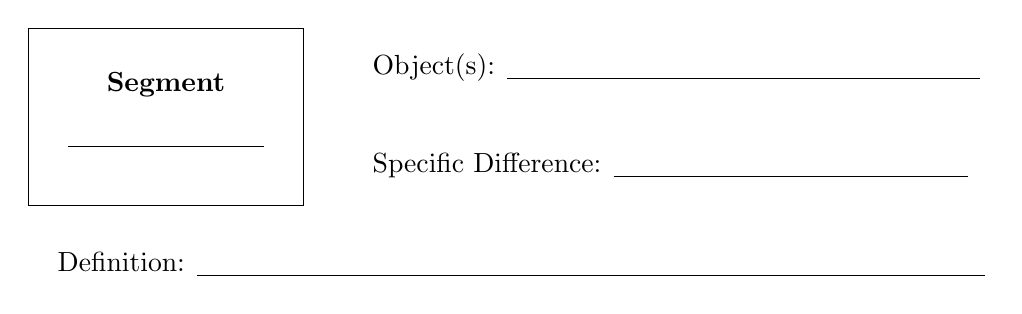
\begin{tikzpicture}
		\coordinate [label=above:{\textbf{Segment}}] 		(A) at (1.5,1);
		\coordinate [label=below:{}] 		(P) at (0.25,0.5);
		\coordinate [label=below:{}] 		(X) at (2.75,0.5);
		\draw (P)--(X);
		\fillpoints{P,X}
		\draw (-0.25,-0.25) rectangle (3.25, 2);
		\coordinate [label=right:{Object(s):  \underline{\hspace{6cm}}}] 		(Y) at (4,1.5);
		\coordinate [label=right:{Specific Difference:  \underline{\hspace{4.5cm}}}] 		(Z) at (4,0.25);
		\coordinate [label=right:{Definition:  \underline{\hspace{10cm}}}] 		(W) at (0,-1);
		
	\end{tikzpicture}
	
	\vspace{0.25cm}
	
	\item \hspace*{4cm} \\ \begin{tikzpicture}
		\coordinate [label=above:{\textbf{Ray}}] 		(A) at (1.5,1);
		\coordinate [label=below:{}] 		(P) at (0.25,0.5);
		\coordinate [label=below:{}] 		(X) at (2.25,0.5);
		\raydraw PX
		\fillpoints{P}
		\draw (-0.25,-0.25) rectangle (3.25, 2);
		\coordinate [label=right:{Object(s):  \underline{\hspace{6cm}}}] 		(Y) at (4,1.5);
		\coordinate [label=right:{Specific Difference:  \underline{\hspace{4.5cm}}}] 		(Z) at (4,0.25);
		\coordinate [label=right:{Definition:  \underline{\hspace{10cm}}}] 		(W) at (0,-1);
		
	\end{tikzpicture}
	
	\vspace{0.25cm}
	
	\item \hspace*{4cm} \\ \begin{tikzpicture}
		\coordinate [label=above:{\textbf{Angle}}] 		(A) at (1.5,1.25);
		\coordinate [label=below:{}] 		(P) at (0.25,0.5);
		\coordinate [label=below:{}] 		(X) at (2.25,1);
		\coordinate [label=below:{}] 		(Y) at (2.25,0);
		\raydraw PX
		\raydraw PY
		\fillpoints{P}
		\draw (-0.25,-0.5) rectangle (3.25, 2);
		\coordinate [label=right:{Object(s):  \underline{\hspace{6cm}}}] 		(M) at (4,1.5);
		\coordinate [label=right:{Specific Difference:  \underline{\hspace{4.5cm}}}] 		(Z) at (4,0.25);
		\coordinate [label=right:{Definition:  \underline{\hspace{10cm}}}] 		(W) at (0,-1.25);
		
	\end{tikzpicture}
	
	\vspace{0.25cm}
	
	\item \hspace*{4cm} \\ 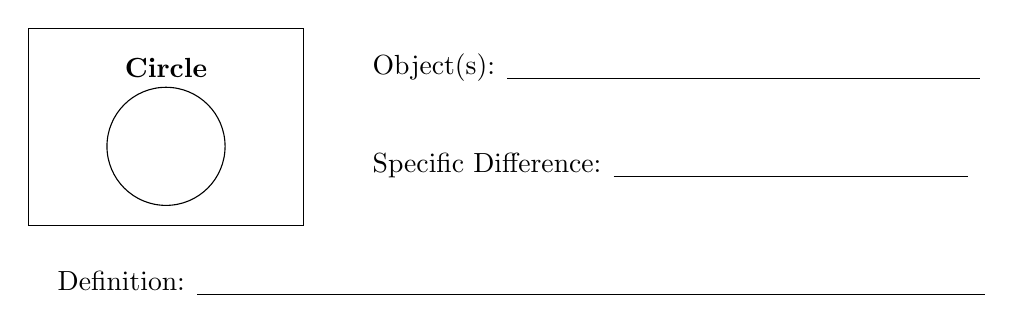
\begin{tikzpicture}
		\coordinate [label=above:{\textbf{Circle}}] 		(A) at (1.5,1.25);
		\coordinate [label=below:{}] 		(P) at (1.5,0.5);
		\coordinate [label=below:{}] 		(X) at (2.25,0.75);
		\coordinate [label=below:{}] 		(Y) at (2.25,0.25);
		\draw (P) circle (.75cm);
		\fillpoints{P}
		\draw (-0.25,-0.5) rectangle (3.25, 2);
		\coordinate [label=right:{Object(s):  \underline{\hspace{6cm}}}] 		(M) at (4,1.5);
		\coordinate [label=right:{Specific Difference:  \underline{\hspace{4.5cm}}}] 		(Z) at (4,0.25);
		\coordinate [label=right:{Definition:  \underline{\hspace{10cm}}}] 		(W) at (0,-1.25);
		
	\end{tikzpicture}
	\end{exparts}
		
	\begin{sol}
	Writing definitions, answers will vary.  
	\end{sol}
	\end{ex}

	
\end{exercises}

%------------------------------------------------------------------------------------
			\section{Elementary objects}
%------------------------------------------------------------------------------------

\subsection{Segment}

A \textbf{segment} is a part of a line that has two \emph{endpoints}.  The \textbf{endpoints} are made where the line is ``cut''.

You should not draw arrows on the end of a segment because, unlike a line, it does not go on forever.

When you name a line segment, use two letters in either order, and put the segment symbol on top.  The segment below could be called \seg XP or \seg PX. 

	\begin{center}
	\begin{tikzpicture}
		\coordinate [label=below:{\pnt P}] 		(P) at (0,0);
		\coordinate [label=below:{\pnt X}] 		(X) at (4,1);
		\draw (P)--(X);
		\fillpoints{P,X}
	\end{tikzpicture}
	\end{center}
	
\q Draw another line segment and name it in two ways.	

\smallskip

\noindent **It is important to note that a segment represents the shortest distance between two points, referred to as ``the distance'' between two points.

\subsection{Ray}

A \textbf{ray} is a part of a line that has one endpoint, and goes on forever in the opposite direction.

Below is a picture of \ray NM.  Note that the endpoint must come first when you are writing the name of a ray.  You could not call it \ray MN. 

	\begin{center}
	\begin{tikzpicture}
		\coordinate [label=below right:{\pnt N}]		(N) at (3,-0.5);
		\coordinate [label=below left:{\pnt M}]		(M) at (0,0);
		\raydraw{N}{M}
		\fillpoints{M,N}
	\end{tikzpicture}
	\end{center}
	
\noindent \q Draw another ray and name it. \aq How could you name the same ray in a different way?\footnote{Place another point on the ray and name the ray with your original endpoint and the new point.}
\medskip

\subsection{Angle}
An \textbf{angle} is two rays with a common endpoint.\footnote{It is important to note that this definition uses objects that we just defined. All of our terms will relate to each other in one way or another.  We have just begun to build!}\\

\newpage

An angle has one \emph{vertex} and two \emph{sides}.
The \textbf{sides} are the two rays that make the angle. 
The \textbf{vertex} is the endpoint they share.

	\begin{center}
	\begin{tikzpicture}
		\coordinate [label=left:{\pnt N}]		(N) at (0,0);
		\coordinate [label=below:{\pnt Y}] 	(Y) at (-25:2);
		\coordinate [label=above:{\pnt X}]	(X) at (10:2.5);
		\coordinate [label=above:{\pnt Z}]	(Z) at (10:3.5);
		\raydraw{N}{Z}
		\raydraw{N}{Y}
		\fillpoints{Y,X,Z}
	\end{tikzpicture}
	\end{center}

For the angle above, the vertex is \pnt N, and the sides are \ray NX and \ray NY.  The angle is named \ang{XNY}. 

When you name an angle, use three letters.  The middle one must be the vertex.  The other two letters must be from both of the two sides.  Remember the angle symbol too.

\noindent \q Name the angle above three other ways.
\medskip

In cases where there is no ambiguity, you may name angles by a single letter representing its vertex.  For example, the angle above could also be named \ang N.

Look at the diagram below.

	\begin{center}
	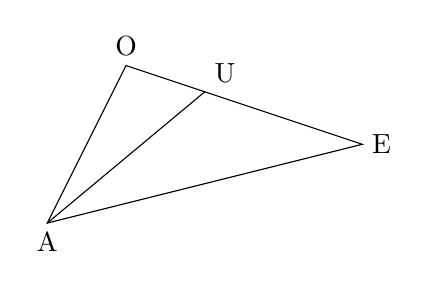
\begin{tikzpicture}
		\draw (0,0) coordinate [label=below:{\pnt A}]	(A)
			-- (4,1) coordinate [label=right:{\pnt E}] (E)
			-- (1,2) coordinate [label=above:{\pnt O}] (O)
			--cycle;
		\draw (A)--(2,{5/3}) coordinate [label=above right:{\pnt U}]	(U);
	\end{tikzpicture}
	\end{center}

\noindent \q Can you write \ang E?  Why or why not?
\vspace{0.75cm}

\noindent \q Can you name all of the angles with vertex \pnt A?
\vspace{0.75cm}

Notice another thing about geometry diagrams:  When a capital letter is near an intersection of two segments, the point is considered to be at that intersection.
Look at \pnt A or \pnt E, for example, in the diagram above.
Even though there are no filled-in dots, the points are still considered to be there.\\\\
**It is also important to note that through any two points, there exists a segment, ray or line, regardless of what is pictured.

\subsection{Circle}

A \textbf{circle} is the set of all points (in a plane) that are the same fixed distance from a given fixed point.  The fixed point is called the \textbf{center}. The fixed distance is called the \textbf{radius}.  It can also be said that all points on the circle are \textbf{equidistant} from the center.  Circles are named using the circle symbol \cir{} and their center.  For example \cir B refers to the circle with center \pnt B.

\noindent \q Label two points on \cir B and draw two radii (plural of radius).\\

\begin{center}
\begin{tikzpicture}

	\coordinate [label=left:$B$] (B) at (0,0);
	\coordinate [label=below:] (A) at (1.5,0);	
%	\draw (O)--(A);	
	\node [draw,circle through=(A)] at (B) {};
	\fill (B) circle (1.5pt);
	
\end{tikzpicture}
\end{center}

While we will study circles extensively later in the course, there are two other terms that will help us communicate in regards to circles.  A \textbf{chord} is a segment connecting any two points on a circle (\seg YZ).  A chord containing the center of a circle (\seg XY) is called the \textbf{diameter}.\\

\begin{center}
\begin{tikzpicture}

	\coordinate [label=below:$O$] (O) at (0,0);
	\coordinate [label=right:$X$] (X) at (1.5,0);	
	\coordinate [label=left:$Y$] (Y) at (-1.5,0);
	\coordinate [label=above right:$Z$] (Z) at (75:1.5);
	\draw (X)--(Y)--(Z);	
	\node [draw,circle through=(X)] at (O) {};
	\fillpoints {O,X,Y,Z}
	
\end{tikzpicture}
\end{center}

\noindent \q  Draw \cir Q with chord \seg AB and diameter \seg AC. \aq Name two segments that have the same length.

\bigskip

\subsection{Locus}

A locus is the set of points that satisfy a particular condition or set of conditions. \aq Place point \pnt R below and sketch the locus of points in a plane one centimeter from \pnt R.  What is this locus?

\smallskip

\subsection{Knowing Definitions}

As you can see, when you are defining a geometric object, it is also important to know what it looks like and how it is written in shorthand with proper notation.

When you ``know'' a term in Geometry, you know these three components:

\begin{enumerate}
\item The words that define it (object(s) and relationship)
\item How to draw it or identify it in a drawing
\item Read and write its notation (shorthand)
\end{enumerate}

It is worth taking the time to carefully understand the definitions, notation and the physical space that an object occupies.  It is essential to be able to identify a term from its picture and/or notation and vice versa, so that we may reason and problem solve with this information later in the course!

\begin{exercises}
	\begin{ex}
	\e Make note cards for the following terms:  \textbf{line} (include collinear), \textbf{segment, ray} (include endpoints), \textbf{angle} (include vertex) and \textbf{circle} (include center, radius, diameter and chord).  See the introduction for details and an example of a complete note card.
	\begin{sol}
	Note cards, answers will vary.  See the introduction for details of what is considered a complete note card  and an example.
	\end{sol}
	\end{ex}
	
	\begin{ex}
	\e Identify the objects below and use proper notation (shorthand) to name them.\\
	(a) \hspace*{\fill} (b) \hspace*{\fill} (c) \hspace*{\fill}\\
	
	\begin{tikzpicture}
		\coordinate [label=below:{\pnt A}]	(M)	at (0,0);
		\coordinate [label=below:{\pnt Z}]	(N)	at (2.5,0);
		\coordinate [label=below:{\pnt B}]	(O)	at (4,0);
		\coordinate [label=below:{\pnt Y}]	(P)	at (6.5,0);
		\coordinate [label=below:{\pnt C}]	(Q)	at (8.5,0);
		\coordinate [label=below:{\pnt X}]	(R)	at (11,0);
		\draw (M)--(N);
		\raydraw OP
		\raydraw RQ
		\fillpoints{M,N,O,P,R,Q}
	\end{tikzpicture}
		
	\vspace{0.25cm}	
	\noindent (d) \hspace*{\fill} (e) \hspace*{\fill}\\
	\begin{tikzpicture}
		\coordinate [label=left:{\pnt J}]	(M)	at (0,0);
		\coordinate [label=below:{\pnt M}]	(N)	at (2.5,0);
		\coordinate [label=above:{\pnt D}]	(O)	at (25:2.5);
		\coordinate [label=below:{\pnt Q}]	(P)	at (7,0.75);
		\coordinate [label=below:{}]		(Q)	at (-1.5,0);
		\coordinate [label=right:{\pnt F}]	(R)	at (7.53,1.28);
		\draw (P) circle (0.75cm);
		\raydraw MN
		\raydraw MO
		\fillpoints{M,N,O,P,R}
	\end{tikzpicture}
	
	\begin{sol}
	\begin{exparts}
	\item Segment AZ, \seg AZ
	\item Ray BY, \ray BY
	\item Ray XC, \ray XC
	\item Angle MJD, \ang MJD
	\item Circle Q, \cir Q
	\end{exparts}
	\end{sol}
	\end{ex}
	
	\begin{ex}
	\e Consider the diagram below:\\
	\begin{center}
	\begin{tikzpicture}
		\coordinate [label=below:{\pnt M}]	(M)	at (0,0);
		\coordinate [label=below:{\pnt N}]	(N)	at (3,0);
		\coordinate [label=below:{\pnt O}]	(O)	at (4,0);
		\coordinate [label=below:{\pnt P}]	(P)	at (6,0);
		\linedraw{M}{P}
		\fillpoints{M,N,O,P}
	\end{tikzpicture}
	\end{center}
	\begin{exparts} 
	\begin{multicols}{2}
	\item Name all the different points.\\\\
	\item Name all the different lines.\\\\
	\item How many possible names are\\ there for the line above?\\
	\item Name all the different segments.\\\\\\
	\item Name all the different rays.\\\\\\
	\end{multicols}
	\end{exparts}
	
	\begin{sol}
		\hspace*{\fill}
		\begin{exparts}
		\item \pnt M, \pnt N, \pnt O, \pnt P
		\item \lin MN
		\item 12
		\item \seg MN,\seg MO, \seg MP, \seg NO, \seg NP, \seg OP
		\item \ray MN, \ray NM, \ray NO, \ray ON, \ray OP, \ray PO
		\end{exparts}
	\end{sol}
	\end{ex}
	
		
	\begin{ex}
	\e Answer each question ``Yes'' or ``No'' based on the diagram below.

	\begin{exparts} \itemsep = \smallskipamount
	\begin{multicols}{2}
	\item Is \pnt C on \lin AB?
	\item Is \pnt C on \lin BC? 
	\item Is \pnt C on \seg AB?
	\item Is \pnt C on \seg BA? 
	\item Is \pnt C on \ray AB?
	\item Is \pnt C on \ray BA?
	\item Is \pnt C on \seg AC?
	\item Is \pnt C on \lin AD? 
	\item Give another name for \ray AB. 
	\item Give two other names for \ang {BAD}.
	\item Are points \pnt A, \pnt B and \pnt C collinear?
	\item Are points \pnt A, \pnt B and \pnt D collinear?
	\end{multicols}
	\end{exparts}
	
	\begin{center}
	\begin{tikzpicture}
		\coordinate [label=below right:\pnt A]	(A)	at (0,0);
		\coordinate [label=below:\pnt B]		(B)	at (3,0);
		\coordinate [label=below:\pnt C]		(C)	at (4,0);
		\coordinate [label=below right:\pnt D]	(D)	at (2,2);
		\linedraw AC
		\linedraw AD
		\fillpoints{A,B,C,D}
	\end{tikzpicture}
	\end{center}

	\begin{sol}
		\hspace*{\fill}
		\begin{exparts} 
			\item Yes
			\item Yes
			\item No
			\item No
			\item Yes
			\item No
			\item Yes
			\item No
			\item \ray AC
			\item \ang {CAD} or \ang {DAB}
			\item Yes
			\item No
		\end{exparts}
	\end{sol}
	\end{ex}
	
	\medskip
	
	\begin{ex}
	
	\e Consider the circle below with center \pnt P.\\
	
	\noindent
	\begin{minipage}{0.3\linewidth}
	
	\begin{tikzpicture}

	\coordinate [label=left:$P$] (B) at (0,0);
	\coordinate [label=above right:$G$] (A) at (60:1.5);
	\coordinate [label=below right:$H$] (C) at (320:1.5);
	\coordinate [label=below left:$K$] (K) at (240:1.5);	
	\draw (K)--(A)--(C)--(B);	
	\node [draw,circle through=(A)] at (B) {};
	\fillpoints{A,B,C,K}
	
	\end{tikzpicture}
	\end{minipage}	
	\begin{minipage}{0.7\linewidth}
	\begin{exparts} \itemsep = \smallskipamount
	\item Use symbolic notation to name the circle.
	\item Name a chord.
	\item Name a diameter.
	\item Name three segments with the same length.
	\end{exparts}
	\end{minipage}
	
	\begin{sol}
		\hspace*{\fill}
		\begin{exparts}
		\item \cir P
		\item \seg GH
		\item \seg GK
		\item \seg PG,\seg PH, \seg PK
		\end{exparts}
	\end{sol}
	\end{ex}
	
	\medskip
		
\end{exercises}

%------------------------------------------------------------------------------------
			\section{Measurement and congruence}
%------------------------------------------------------------------------------------

\subsection{Measurement}
Segments and angles can be measured. 
Lines and rays cannot (why not?).

Segments are measured with a ruler. 
You can use inches, centimeters, or any other convenient unit.

To indicate the measure of a segment, omit the segment symbol. 
For example, you would write $AB = 5$\,cm.\footnote{This reads: ''The distance between A and B is 5 cm.''} 
It is ok if you accidentally write the segment symbol; it will be understood what you mean.

Angles are measured with a protractor. 
We will measure angles in degrees.

To indicate the measure of an angle, use a lowercase ``m''. 
For example, you would write m$\ang{XAQ} = 41\degree$.
It is ok if you forget the ``m''; it will be understood what you mean.\\

\noindent \q Measure the length of \seg XY  in centimeters and \ang DEF in degrees.

\begin{center}
	\begin{tikzpicture}
		\coordinate [label=below:\pnt X]		(B)	at (-5.5,0);
		\coordinate [label=below:\pnt Y]		(E)	at (-2.0,0);
	
		\coordinate [label=below left:\pnt E]	(A)	at (0,0);
		
		\coordinate [label=below:\pnt D]		(C)	at (4,0);
		\coordinate [label=above left:\pnt F]	(D)	at (35:4);
		
		\coordinate [label=above left:]	(P)	at (34:2);		
		\coordinate [label=above left:]	(Q)	at (1:2);
		\draw [red, latex-latex] (P) arc (34:1:2) node [pos=0.5, right] {\angm DEF};
		
		\raydraw AC
		\raydraw AD
		\draw (B)--(E);
		\fillpoints{A,B,C,D,E}
	\end{tikzpicture}
	\end{center}

\subsection{Angle measure classifications}
\noindent A \textbf{right angle} is an angle whose measure is $90\degree$.\\
A \textbf{straight angle} is an angle whose measure is $180\degree$.\\
An \textbf{acute angle} is an angle whose measure is less than $90\degree$.\\
An \textbf{obtuse angle} is an angle whose measure is more than $90\degree$ and less than $180\degree$.\\
A \textbf{reflex angle} is an angle whose measure is more than $180\degree$ and less than $360\degree$.\\

\noindent \q Sketch, with a straight edge, an example of each of the first 4 angle classifications.  Measure the acute and obtuse angles.  Label a reflex angle on either the acute or obtuse angle.

\vfill


\paragraph{Course Assumption}
When you are asked for the measure of an angle it can be assumed it is a measure of $180\degree$ or less.  You may also assume when an angle is named, it refers to an angle of $180\degree$ or less.

\paragraph{Course Assumption}
You may assume if an object appears to be a line it is a line.  Consequently, if an angle appears to be a straight angle, it is a straight angle.

\subsection{Congruence}
If two segments (or two angles) have the same measure, then they are called \textbf{congruent}.  The symbol for congruent is $\cong$.  When you express that two objects (segments, angles, triangles, etc.) are congruent, this is called a \textbf{congruence statement}.  For example, consider this diagram where $\segl HI = 4$\,cm and $\segl FJ = 4$\,cm:

	\begin{center}
	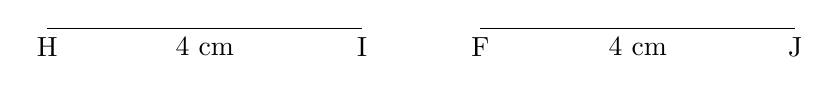
\begin{tikzpicture}
		\coordinate [label=below:\pnt H]		(B)	at (-5.5,0);
		\coordinate [label=below:\pnt I]		(E)	at (-1.5,0);
		\coordinate [label=below:\pnt F]		(A)	at (0,0);
		\coordinate [label=below:\pnt J]		(C)	at (4,0);
		\draw (B)--(E) node [below, pos=0.5] {4~cm};
		\draw (A)--(C) node [below, pos=0.5] {4~cm};
		\fillpoints{A,B,C,E}
	\end{tikzpicture}
	\end{center}

\noindent We could write a \emph{congruence statement}:  \segcong{HI}{FJ}

\newpage

\noindent Or consider this diagram where $\angm{ABC} =40\degree$ and $\angm {DEF}=40\degree$:

	\begin{center}
	\begin{tikzpicture}
		\coordinate [label=below left:\pnt B]	(B)	at (0,0);
		\coordinate [label=below:\pnt C]		(C)	at (3,0);
		\coordinate [label=above left:\pnt A]	(A)	at (40:3);
		\coordinate [label=above right:40\degree]	(P)	at (0.5,0);
		
		\begin{scope} [xshift=5cm]
		\coordinate [label=below left:\pnt E]	(E)	at (0,0);
		\coordinate [label=below:\pnt D]		(D)	at (3,0);
		\coordinate [label=above left:\pnt F]	(F)	at (40:3);
		\coordinate [label=above right:40\degree]	(Q)	at (0.5,0);
		\end{scope}
				
		\raydraw BC
		\raydraw BA
		\raydraw ED
		\raydraw EF
		\fillpoints{A,C,D,F}
	\end{tikzpicture}
	\end{center}
	
\noindent We could write a \emph{congruence statement}:  \angcong{ABC}{DEF}
\smallskip	

In diagrams, congruence is demonstrated with \emph{tick marks} shown in the diagram below.  **When you know it, you should always mark congruence on your diagrams!

	\begin{tikzpicture} 
		\coordinate [label=below:]		(B)	at (0,0);
		\coordinate [label=below:]		(E)	at (2,0);
		\coordinate [label=below:]		(A)	at (3,0);
		\coordinate [label=below:]		(C)	at (5,0);
		\draw (B)--(E) node [below, pos=0.5] {};
		\draw (A)--(C) node [below, pos=0.5] {};
		\fillpoints{A,B,C,E}
		\tick BEAC
	\end{tikzpicture}
	\begin{tikzpicture} 
		\coordinate [label=below left:]	(B)	at (0,0);
		\coordinate [label=below:]		(C)	at (1.5,0);
		\coordinate [label=above left:]	(A)	at (40:1.5);
		\coordinate [label=above right:]	(P)	at (-1.5,0);
		
		\begin{scope} [xshift=3cm]
		\coordinate [label=below left:]	(E)	at (0,0);
		\coordinate [label=below:]		(D)	at (1.5,0);
		\coordinate [label=above left:]	(F)	at (40:1.5);
		\coordinate [label=above right:]	(Q)	at (0.5,0);
		\end{scope}
				
		\raydraw BC
		\raydraw BA
		\raydraw ED
		\raydraw EF
		\mmangle BCA
		\mmangle EDF
	\end{tikzpicture}
	
	When two objects are \emph{not congruent}, the symbol, $\not\cong$, is used to express it in notation.  In fact, drawing a slash from top right to bottom left negates the meaning of many mathematical symbols.

\smallskip	

\noindent \q In the diagrams below, measure $\angle KLM$ and $XY$.  Then place point \pnt Z on \ray XY so that \segcong{XY}{YZ}.  Then draw \ray LN, where \pnt N is not on \ray LM, so that \angcong{KLM}{NLK}.

\medskip

\noindent
	\begin{tikzpicture}
		\coordinate [label=left:\pnt L]		(L) at (0,0);
		\coordinate [label=above left:\pnt K]	(K) at (60:4);
		\coordinate [label=below:\pnt M] 	(M) at (10:4);
		\coordinate [label=below:\pnt X]	(X) at (5.5,0);
		\coordinate [label=below:\pnt Y]	(Y) at (7.8,0);
		\coordinate [label=below:] 			(Z) at (11,0);
		\raydraw LK;
		\raydraw LM;
		\raydraw XZ;
		\fillpoints{L,K,M,X,Y}
	\end{tikzpicture}

	
\noindent \q Classify $\angle KLM$ and $\angle NLM$ as acute, right, obtuse or straight.	

\medskip

\begin{exercises}
	\begin{ex}
	\e Make note cards for:  \textbf{angle measurement classifications} (include examples) and \textbf{congruence} (include congruence statement).  
	\begin{sol}
	Note cards
	\end{sol}
	\end{ex}
	
	\begin{ex}
	\e Give the measure of the following angles:
	
	\noindent
	\begin{tikzpicture}
		\coordinate [label=below:\pnt R]	(L) at (0,0);
		\coordinate [label=above:]			(K) at (120:3);
		\coordinate [label=below:] 			(M) at (3,0);
		\coordinate [label=below:\pnt X]	(X) at (4.5,0);
		\coordinate [label=below:]			(Y) at (7.5,0);
		\coordinate [label=below:] 			(Z) at (7,2);
		\coordinate [label=below:\pnt T]	(T) at (9,0);
		\coordinate [label=below:]			(U) at (11,1);
		\coordinate [label=below:] 			(V) at (8,2);
		\raydraw LK;
		\raydraw LM;
		\raydraw XY;
		\raydraw XZ;
		\raydraw TU;
		\raydraw TV;
	\end{tikzpicture}
	\begin{sol}
	$\angm{R} =120\degree$, $\angm{X} =38.7\degree$, $\angm{T} =90\degree$
	\end{sol}
	\end{ex}
	

	\begin{ex}
	\e Use the diagram below to answer the questions that follow.
	\begin{center}
	\begin{tikzpicture}
		\coordinate [label=left:\pnt A]		(A) at (0,0);
		\coordinate [label=right:\pnt B]	(B) at (-32:4.4);
		\coordinate [label=above:\pnt D] 	(D) at (67:2.4);
		\coordinate [label=above right:\pnt J] (J) at ($(D)!3.1cm!99:(A)$);
		\coordinate [label=right:\pnt K] 	(K) at ($(D)!.75!(B)$);
		\draw (A)--(B)--(D)--cycle;
		\draw (D)--(J)--(B);
		\fillpoints{K}
	\end{tikzpicture}
	\end{center}
	
	\begin{exparts}
	\item Find the lengths of \seg AB and \seg BD in centimeters.
	
	\item Find \angm{ABD}. 
	
	\item Is \ang{ABD} acute, right, obtuse, or straight?
	
	\item Does \ang{BAD} look acute, right, obtuse, or straight? 
	Use your protractor to find its measure and check your choice.
	
	\item  Measure \ang ADJ.
		If \ang ADJ is congruent to another angle in the diagram,
		write a congruence statement.

	\item Name a straight angle in the figure.
	
	\end{exparts}

	\begin{sol}
	\begin{exparts}
	\item $\segl AB=4.4$, $\segl BD=5.3$
	\item 26.4\degree
	\item acute
	\item obtuse, $\approx 99\degree$
	\item $\angm {ADJ}\approx 99\degree$, so $\angcong{ADJ}{BAD}\cong \angle DJB$
	\item \ang {DKB}
	\end{exparts}
	\end{sol}
	\end{ex}
	
		\begin{ex}
	\e Using a protractor, draw angles of measure 35\degree, 90\degree and 140\degree. Then label each angle as acute, right or obtuse.
	\begin{sol}
	Diagrams will vary
	\end{sol}
	\end{ex}
	
	\bigskip
	
	\begin{ex}
	\e Now that we have definitions for a small group of elementary objects, let's begin to define some of the terms that will be used in our reasoning later in the course.  For the four terms (perpendicular, segment bisector, angle bisector and midpoint), the term and a drawing are given.  As we have done before, write the object(s) involved and the specific difference that this object has from the original parts that comprise it.  Then write a sentence that links the object(s) and the specificity.\\
	
	\begin{exparts}	
	\item \hspace*{4cm} \\ 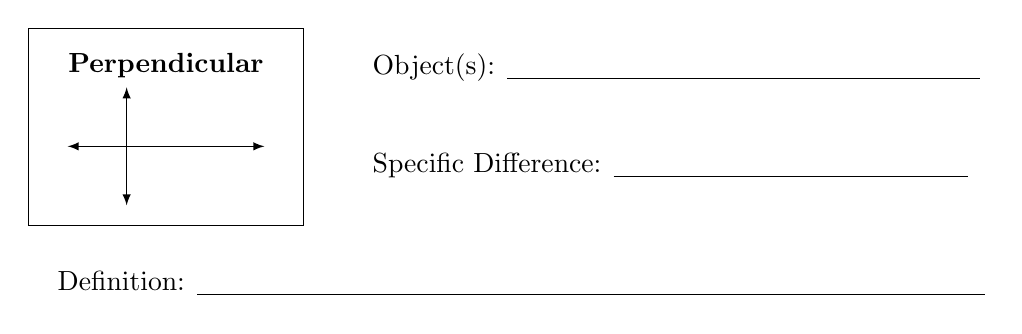
\begin{tikzpicture}
		\coordinate [label=above:{\textbf{Perpendicular}}] 		(A) at (1.5,1.25);
		\coordinate [label=below:{}] 		(P) at (0.25,0.5);
		\coordinate [label=below:{}] 		(X) at (2.75,0.5);
		\coordinate [label=below:{}] 		(B) at (1,1.25);
		\coordinate [label=below:{}] 		(C) at (1,-0.25);
		\draw [latex-latex] (P)--(X);
		\draw [latex-latex] (B)--(C);
		\perpbox {1,0.5}XB
		\draw (-0.25,-0.5) rectangle (3.25, 2);
		\coordinate [label=right:{Object(s):  \underline{\hspace{6cm}}}] 		(Y) at (4,1.5);
		\coordinate [label=right:{Specific Difference:  \underline{\hspace{4.5cm}}}] 		(Z) at (4,0.25);
		\coordinate [label=right:{Definition:  \underline{\hspace{10cm}}}] 		(W) at (0,-1.25);
		
	\end{tikzpicture}
	
	\vspace{0.25cm}
	
	\item \hspace*{4cm} \\ 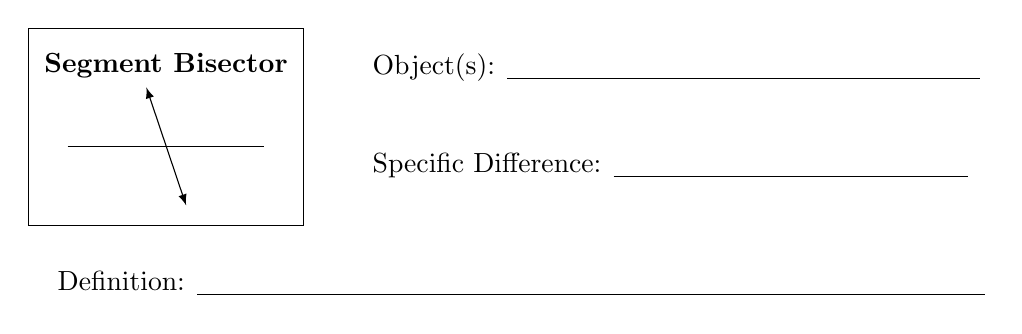
\begin{tikzpicture}
		\coordinate [label=above:{\textbf{Segment Bisector}}] 		(A) at (1.5,1.25);
		\coordinate [label=below:{}] 		(P) at (0.25,0.5);
		\coordinate [label=below:{}] 		(X) at (2.75,0.5);
		\coordinate [label=below:{}] 		(B) at (1.25,1.25);
		\coordinate [label=below:{}] 		(C) at (1.755,-0.25);
		\draw (P)--(X);
		\draw [latex-latex] (B)--(C);
		\ttick P{1.5,0.5}{1.5,0.5}X
		\fillpoints {P,X}
		\draw (-0.25,-0.5) rectangle (3.25, 2);
		\coordinate [label=right:{Object(s):  \underline{\hspace{6cm}}}] 		(Y) at (4,1.5);
		\coordinate [label=right:{Specific Difference:  \underline{\hspace{4.5cm}}}] 		(Z) at (4,0.25);
		\coordinate [label=right:{Definition:  \underline{\hspace{10cm}}}] 		(W) at (0,-1.25);
		
	\end{tikzpicture}
	
	\vspace{0.25cm}
	
	\item \hspace*{4cm} \\ 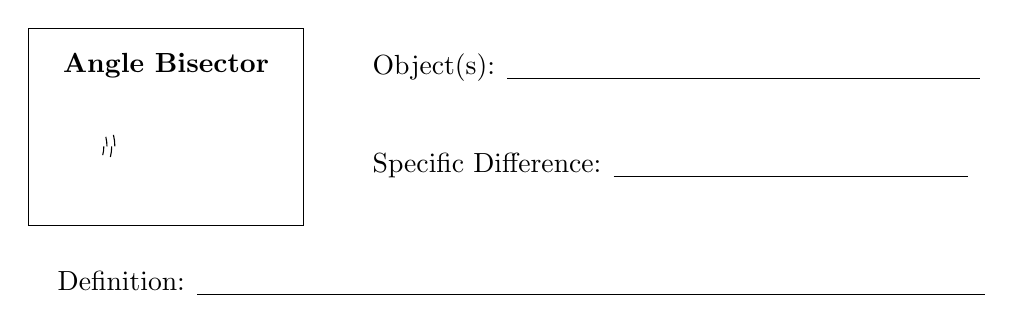
\begin{tikzpicture}
		\coordinate [label=above:{\textbf{Angle Bisector}}] 		(A) at (1.5,1.25);
		\coordinate [label=below:{}] 		(P) at (0.25,0.5);
		\coordinate [label=below:{}] 		(X) at (2.25,1);
		\coordinate [label=below:{}] 		(Y) at (2.25,0);
		\coordinate [label=below:{}] 		(Z) at (2.25,0.5);
		\raydraw PX
		\raydraw PY
		\raydraw PZ
		\fillpoints{P}
%		\mangle PZX
%		\mangleoffset PYZ
			\path  (P)-- +(0:0.5) coordinate (m3); 
			\path  (P)-- +(0:0.6) coordinate (m4);
			\draw (m3) arc (0:14:0.5);
			\draw (m4) arc (0:14:0.6);
			
			\path  (P)-- +(0:0.46) coordinate (m5); 
			\path  (P)-- +(0:0.56) coordinate (m6);
			\draw (m5) arc (0:-14:0.46);
			\draw (m6) arc (0:-14:0.56);
		\draw (-0.25,-0.5) rectangle (3.25, 2);
		\coordinate [label=right:{Object(s):  \underline{\hspace{6cm}}}] 		(M) at (4,1.5);
		\coordinate [label=right:{Specific Difference:  \underline{\hspace{4.5cm}}}] 		(N) at (4,0.25);
		\coordinate [label=right:{Definition:  \underline{\hspace{10cm}}}] 		(O) at (0,-1.25);
		
	\end{tikzpicture}
	
	\vspace{0.25cm}
	
	\item \hspace*{4cm} \\ 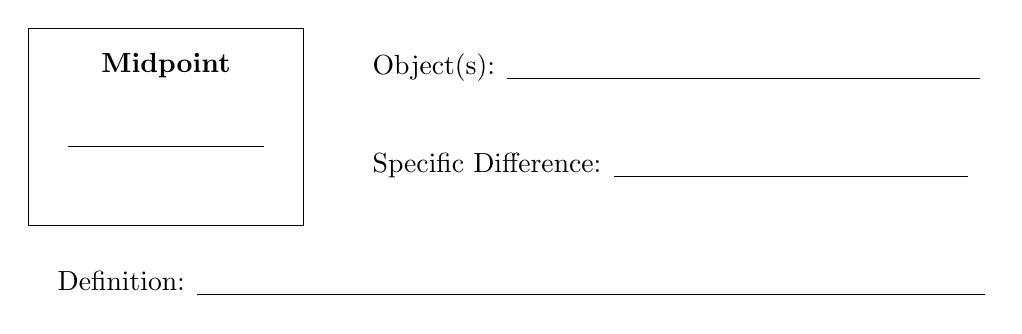
\begin{tikzpicture}
		\coordinate [label=above:{\textbf{Midpoint}}] 		(A) at (1.5,1.25);
		\coordinate [label=below:{}] 		(P) at (0.25,0.5);
		\coordinate [label=below:{}] 		(X) at (2.75,0.5);
		\coordinate [label=below:{}] 		(B) at (1.5,0.5);
		\draw (P)--(X);
		\fillpoints{P,X,B}
		\ttick PBBX
		\draw (-0.25,-0.5) rectangle (3.25, 2);
		\coordinate [label=right:{Object(s):  \underline{\hspace{6cm}}}] 		(P) at (4,1.5);
		\coordinate [label=right:{Specific Difference:  \underline{\hspace{4.5cm}}}] 		(X) at (4,0.25);
		\coordinate [label=right:{Definition:  \underline{\hspace{10cm}}}] 		(X) at (0,-1.25);
		
	\end{tikzpicture}
	\end{exparts}
		
	\begin{sol}
	Writing definitions, answers will vary.  
	\end{sol}
	\end{ex}
	
\end{exercises}

%------------------------------------------------------------------------------------
			\section{Advanced:  Constructions}
%------------------------------------------------------------------------------------

In geometry, a \emph{construction} is a (relatively) precise method of creating geometry diagrams that uses only two tools.  The tools are a \emph{straightedge} (not a ruler), and a \emph{compass} (not a protractor).

When you are asked to \textbf{construct} an object, you should use a straightedge and compass to make your drawing as precise as possible.  In contrast, when you are asked to \textbf{sketch} an object you can use---or not use---whatever tools you want. Most people just ``eyeball'' the drawing so it looks close enough, but other people like to use rulers or protractors so they are as clean as possible. \q What is the difference between the instructions \emph{construct} and \emph{sketch}?

\newpage

\subsection{Construct a Circle}
The goal is to construct a circle with a given radius.  Segment $\overline{OA}$ is below. \q Construct $\odot O$ that has radius $OA$.

\vspace{1.25cm}

\begin{center}
\begin{tikzpicture}

	\coordinate [label=below:$O$] (O) at (0,0);
	\coordinate [label=below:$A$] (A) at (2.5,0);	
	\draw (O)--(A);	
%	\node [draw,circle through=(Y)] at (X) {};
	\fillpoints {A,O} 
	
\end{tikzpicture}
\end{center}

\vspace{1cm}

\noindent \q What does a compass do?

\subsection{Duplicate a Segment}
The goal is to construct a segment that is congruent to a given segment.  Segment \seg PQ is below. \q Construct a segment, \seg AB that is congruent to \seg PQ.

\begin{enumerate}
\item Use your straightedge to draw a line segment longer than the one to be duplicated.
\item Label one of the new endpoints (usually on one end).
\item Open your compass up to the size of the segment to be duplicated.  Put the pin on the new endpoint and mark where the other endpoint should be.  Label the other endpoint! (Mark congruent parts)
\end{enumerate}

\begin{tikzpicture}

	\coordinate [label=below:$P$] (O) at (0,0);
	\coordinate [label=below:$Q$] (A) at (4,0);	
	\draw (O)--(A);	
%	\node [draw,circle through=(Y)] at (X) {};
	\fillpoints {A,O}
	
\end{tikzpicture}

\medskip

\subsection{Duplicate an Angle}
**Very important:  Any line can be drawn, but a ``particular'' line must have two points to define it!\\

The goal is to construct an angle that is congruent to a given angle.  $\angle YXZ$ is below. \q Construct an angle \ang DEF that is congruent to $\angle YXZ$.

\begin{enumerate}
\item Use your straight edge to draw a ray.  Mark the new vertex on the endpoint of the ray.
\item Open your compass up to any size.  Place the pin on the original vertex and make a ``reference'' arc that spans the original angle.
\item Put the pin on the new vertex and make the same reference arc on the new ray.  Make sure that there is enough arc on either side of the ray to span the angle to be duplicated.
\item Open your compass up to the distance between the original arc's intersection points with the sides of the angle.  Place the pin of the compass on the new intersection point between arc and ray.
\item Mark the distance on the arc.  Make a ray from the vertex, through this point.  Label points on the angle. (Mark congruent parts)
\end{enumerate}

	\begin{tikzpicture}
		\coordinate [label=below left:{$X$}]		(X) at (0,0);
		\coordinate [label=below:{$Y$}] 			(Y) at (0:3);
		\coordinate [label=above left:{$Z$}]		(Z) at (40:3.5);
		\raydraw{X}{Z}
		\raydraw{X}{Y}
		\fillpoints{Y,X,Z}
	\end{tikzpicture}
	
\smallskip	

\noindent \q The goal is to construct an angle that is the sum of two angles.  $\angle YXZ$ is above. Construct an angle, $\angle QRS$, that has twice the measure of $\angle YXZ$.

\bigskip

\begin{exercises}

\begin{ex}
In the space below, use a straight edge to sketch an angle that looks obtuse. Then, duplicate it.
\bigskip
\begin{sol}
Construction
\end{sol}
\end{ex}

\begin{ex}

Consider the three segments drawn below.

\begin{tikzpicture}

	\coordinate [label=below:$A$] (A) at (0,0);
	\coordinate [label=below:$B$] (B) at (5,0);	
	\coordinate [label=left:$C$] (C) at (6,2);
	\coordinate [label=below:$D$] (D) at (8,0);	
	\coordinate [label=below:$E$] (E) at (9,2);
	\coordinate [label=below:$F$] (F) at (11,2);			
	\draw (A)--(B);	
	\draw (C)--(D);
	\draw (E)--(F);		
	\fillpoints{A,B,C,D,E,F}

	
\end{tikzpicture}

\begin{exparts}
\item Duplicate each of the three segments.
\bigskip
\item Construct a new segment $\overline{MN}$ that has length $AB+2CD$.
\vspace{1.5cm}
\item Construct a new segment $\overline{TU}$ that has length $AB - EF$.
\vspace{1.5cm}
\end{exparts}
\begin{sol}
Constructions
\end{sol}
\end{ex}

\begin{ex}
Consider the two angles drawn below.  Construct a new angle $\angle ABC$ that has measure m$\angle GHI + \text{m}\angle JKL$.

	\begin{tikzpicture}
		\coordinate [label=left:{$H$}]		(H) at (0,0);
		\coordinate [label=below:{$G$}] 	(G) at (0:3);
		\coordinate [label=above:{$I$}]		(I) at (30:3.5);
		\raydraw{H}{G}
		\raydraw{H}{I}
		\coordinate [label=left:{$J$}]		(J) at (6,3);
		\coordinate [label=below:{$K$}] 	(K) at (7,0);
		\coordinate [label=right:{$L$}]		(L) at (9,3);
		\raydraw{K}{J}
		\raydraw{K}{L}
		\fillpoints{G,H,I,J,K,L}
	\end{tikzpicture}

\vfill
\begin{sol}
Construction
\end{sol}
\end{ex}

\end{exercises}

\newpage

%--------------------------------------------------------------------------
			\section{Perpendiculars and bisectors}
%--------------------------------------------------------------------------

\subsection{Perpendicular}
Two lines (segments/rays) are \textbf{perpendicular} if they meet at right angles.  In writing, the symbol for ``perpendicular to'' is $\perp$.

In a diagram, a little square is used to show that two lines are perpendicular. 
The little square in the diagram below tells you that \segperp {TS}{WV}.

	\begin{center}
	\begin{tikzpicture}
		\coordinate [label={[shift={(-.2,-.6)}] \pnt C}]	(C)	at (0,0);
		\coordinate [label=above:\pnt V]			(V)	at (110:1.5);
		\coordinate [label=below:\pnt W]			(W)	at (-70:1.5);
		\coordinate [label=left:\pnt S]				(S)	at (200:2);
		\coordinate [label=right:\pnt T]				(T)	at (20:3);
		\draw (S)--(T);
		\draw (V)--(W);
		\perpbox CTV
	\end{tikzpicture}
	\end{center}

\noindent **If you do not see the little square, you should not assume that the lines are perpendicular!\\

\noindent \q In the space below, sketch a picture in which \segperp{BD}{PQ}.  Mark your diagram.
\bigskip

\noindent \q Did you mark your diagram with the little square? Why is it important to mark your diagram?
\smallskip

\subsection{Distance from a point to a line}

A quick word about distance:  the distance between two points is probably obvious,
but the distance between a point and a line may not be.\\

\newpage

Depending on how you place your ruler, you could seemingly have many different answers.

	\begin{center}
	\begin{tikzpicture}[font=\scriptsize]
		\coordinate [label=left:{\normalsize \pnt P}] (P) at (0,0);
		\coordinate (a) at (-90:2);
		\coordinate (b) at (10:3);
		\coordinate (c) at (-49.5:1.52);
		\begin{scope}[dashed, thick]
			\draw (P) -- (c) node [midway,above right] {1.52};
			\draw (P) -- (a) node [midway,left] {2} node [pos=1,right] {\pnt A};
			\draw (P)--(b) node [midway,above] {3} node [pos=1,below] {\pnt B};
		\end{scope}
		\linedraw ab
		\perpbox cbP
		\fillpoints {P,a,b}
	\end{tikzpicture}
	\end{center}

The convention is to define the distance between a point and a line to be the \textit{perpendicular distance} (or shortest distance).  In the diagram above, \pnt P is 1.52 units from \lin AB.

\subsection{Midpoints and bisectors}

To \textbf{bisect} something means to cut into two congruent parts.  You can bisect a segment or an angle.  \q You cannot bisect a line or ray (why not?).\\

Reminder:  In a diagram, you show that an object is bisected by putting identical \emph{tick marks} on the two congruent pieces. In diagrams where there are more than one set of congruent segments or angles, use one, two and three tick marks to differentiate between congruent pairs of parts.\\

In the diagram below, \seg DC bisects \seg AB and \ray CE bisects \ang{ACD}.  (Notice that sometimes you offset the tick marks on angles so it doesn't look like one big mark.)

\q Are there any other bisecting statements that could be made about this drawing?

	\begin{center}
	\begin{tikzpicture} [scale=0.9]
		\coordinate [label=above:{\pnt C}]	(C) at (0,0);
		\coordinate [label=above:{\pnt A}]	(A) at (-10:2);
		\coordinate [label=right:{\pnt E}]	(E) at (-80:2);
		\coordinate [label=above:{\pnt B}]	(B) at (170:2);
		\coordinate [label=left:{\pnt D}]	(D) at (-150:3.5);
		\tick{B}{C}{C}{A}
		\draw (C)--(B)--(D)--cycle;
		\draw [latex-] (E)--(C)--(A);
%		\mmangle CECA
%		\mmangleoffset CDCE
		\draw ($(C)!.25cm!(E)$) arc (-80:-10:.25cm); 
		\draw ($(C)!.3cm!(E)$) arc (-80:-10:.3cm); 
		\draw ($(C)!.28cm!(D)$) arc (-150:-80:.28cm); 
		\draw ($(C)!.33cm!(D)$) arc (-150:-80:.33cm); 
	\end{tikzpicture}
	\end{center}

\noindent \q What happens if two angles seem like they are congruent, but do not have the tick marks?
\smallskip

Every segment has a \textbf{midpoint} that divides it into two congruent segments. \q Lines and rays do not have midpoints. (Why not?)\\
\smallskip

In the diagram below, \pnt D is the midpoint of \seg XY.  Again, the identical tick marks help you see that \segcong{XD}{DY}.\\

	\begin{center}
	\begin{tikzpicture}
		\coordinate [label=below:\pnt X]			(X)	at (0,0);
		\coordinate [label=below:\pnt Y]			(Y)	at (4,0);
		\coordinate [label=below:\pnt D]			(D)	at ($(X)!.5!(Y)$);
		\draw (X)--(Y);
		\fillpoints{X,D,Y}
		\tick XDDY
	\end{tikzpicture}
	\end{center}
	
\noindent \q In the space below, draw \seg AZ through \pnt Y, such that \pnt Y is the midpoint of \seg AZ.  Mark your diagram.

	\begin{center}
	\hspace*{4cm}
	\begin{tikzpicture}
		\coordinate [label=below:{\pnt Y}]			(Y)	at (0,0);
		\coordinate [label=below:{\pnt A}]			(A)	at (3,1);
		\fillpoints{A,Y}
	\end{tikzpicture}
	\end{center}
\bigskip

\noindent \q Did you mark your diagram with the tick marks?  Why is it important to mark your diagram?
\medskip

\noindent **Once you have a diagram, you can use your algebra skills to problem solve.
\q For example,
if you are given that $\segl ZA =12$ and $\segl YZ=x+1$,
can you solve for $x$?
\bigskip

\noindent \q If a segment is bisected, it must be bisected at its midpoint. (Why?)
\medskip
\newpage

By the way, you use tick marks any time a diagram has congruent segments, not just if there are midpoints and bisectors.  Below is an example of an object with two pairs of congruent segments.  Note, a different number of tick marks are used for each pair to show that they are not all congruent to each other.

	\begin{center}
	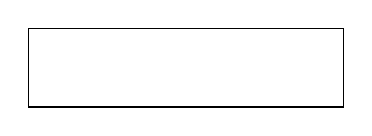
\begin{tikzpicture}
		\coordinate 			(A)	at (0,0);
		\coordinate 			(B)	at (4,0);
		\coordinate 			(C)	at (4,1);
		\coordinate 			(D)	at (0,1);
		\draw (A)--(B)--(C)--(D)--cycle;
		\tick ABCD
		\ttick ADBC
	\end{tikzpicture}
	\end{center}
	
\paragraph{Course Convention}	
As diagrams get more complex, it is important to understand the conventions used in this text.  Capital letters refer to points.  Lowercase letters refer to unknown variables.  If a variable (or variable expression) \emph{does not} have degrees ($^\circ$) symbol (ex: $3a+5$), then you are solving for a length.  If a variable \emph{does} have a degrees symbol (ex: $a^\circ$), then you are solving for an angle measure.

\smallskip

\noindent \q In the diagram below, find $a$ and $b$.\footnote{$a=90$, $b=\frac{3}{2}$}\\

	\begin{tikzpicture}
		\coordinate [label={[shift={(-.2,-.7)}] \pnt X },
					label={{[shift={(.35,-.35)}] \footnotesize $a\degree$ }} ]	
										(X) at (0,0);
		\coordinate [label=above right:\pnt V]	(V) at (20:1.5);
		\coordinate [label=below left:\pnt W]		(W) at (200:1.5);
		\coordinate [label=above:\pnt Y]		(Y) at (110:1);
		\coordinate [label=below:\pnt Z]		(Z) at (290:3);
		\draw (Y)--(Z);
		\draw (W)--(X) node [midway,sloped,above=2pt] {\footnotesize $3b+7$} 
			-- (V) node [midway,sloped,above=2pt] {\footnotesize $5b+4$};
		\perpbox XVY
		\ttick WXXV
	\end{tikzpicture}
	
\noindent \q Write, in words, a description of the diagram above.\footnote{\seg YZ is perpendicular to  \seg WV and bisects  \seg WV}

\medskip
\newpage

\subsection{Perpendicular bisector}
\label{sec:perp-bis}

The \textbf{perpendicular bisector} of a segment is a line that bisects the segment, and is perpendicular to it. \q Only a segment can have a perpendicular bisector. (Why?)

Look back at the question on the previous page.  It is most easily answered as
\emph{\seg YZ is the perpendicular bisector of \seg WV}.

\noindent \q Sketch a diagram in which \seg JH is the perpendicular bisector of \seg KL.  Which of the following must be true?  (Hint: Only three of them must be true.)

\begin{enumerate}
\item \segperp {JH}{KL}
\item \segperp {KL}{JH}
\item \segbis {JH}{KL}
\item \segbis{KL}{JH}
\end{enumerate}

\paragraph{Naming Lines}
We have named lines with two letters, for example: \lin AB.  It is also common in geometry to name lines with a lower case letter (found near an arrow at one of the ends).  The most common letters used for line naming are $\ell$, $m$, $n$ and $k$.

\paragraph{Exploration:  Perpendicular Bisector}
Consider the diagram below where line $\ell$ is the perpendicular bisector of \seg AB, and follow the directions below:\\

\begin{multicols}{2}
\begin{enumerate}
\item Choose any point \pnt P on $\ell$. 
Measure the distances \segl PA and \segl PB.

\item Choose a different point \pnt Q on $\ell$.
Measure the distances \segl QA and \segl QB.

\item Make a conjecture about a segment and its perpendicular bisector.
\end{enumerate}
	\begin{flushright}
	\begin{tikzpicture}
		\coordinate [label=right:]				(X) at (0,0);
		\coordinate [label=above right:$\ell$]			(V) at (0,3);
		\coordinate [label=left:]				(W) at (0,-3);
		\coordinate [label=below:\pnt A]		(A) at (-2,0);
		\coordinate [label=below:\pnt B]		(B) at (2,0);
		\draw (A)--(B);
		\linedraw VW
		\perpbox XBV
		\ttick AXXB
		\fillpoints{A,B}
	\end{tikzpicture}
	\end{flushright}
\end{multicols}
\medskip
\newpage

\subsection{Summary}

The perpendicular bisector (theorem) is widely used in geometry.  We will discuss \emph{theorems} later in the course and we will prove this theorem later, as well.  

\begin{tcolorbox}
\textbf{Perpendicular Bisector (theorem)}
\begin{center}
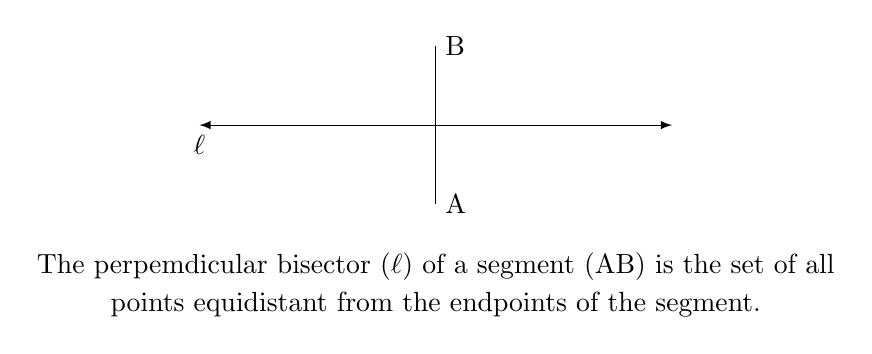
\begin{tikzpicture}

	\coordinate[label=below:{}]				(X)	at	(2,1);
	\coordinate[label=right:{\pnt A}]				(A)	at	(2,0);
	\coordinate[label=right:{\pnt B}]				(B)	at	(2,2);
	\coordinate[label=below:{$\ell$}]				(C)	at	(-1,1);
	\coordinate[label=below:{}]				(F)	at	(5,1);
	\coordinate[label=below:{The perpemdicular bisector ($\ell$) of a segment (\seg AB) is the set of all}]				(D)	at	(2,-0.5);
	\coordinate[label=below:{points equidistant from the endpoints of the segment.}]				(E)	at	(2,-1);
	\fillpoints {A,B}
	\draw (A)--(B);
	\draw [latex-latex] (C)--(F);
	\ttick AXXB
	\perpbox XFB
	
\end{tikzpicture}
\end{center}
\end{tcolorbox}

Here are two postulates to consider when solving and reasoning through problems:

\begin{tcolorbox}
\textbf{Segment Addition postulate} \\
\begin{center}
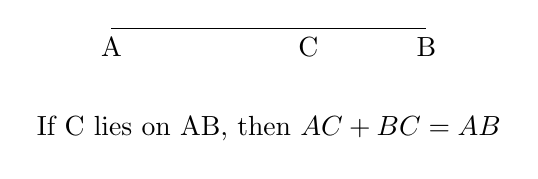
\begin{tikzpicture}

	\coordinate[label=below:{\pnt{A}}]				(A)	at	(0,0);
	\coordinate[label=below:{\pnt{B}}]				(B)	at	(4,0);
	\coordinate[label=below:{\pnt{C}}]				(C)	at	(2.5,0);
	\coordinate[label=below:{If \pnt C lies on \seg AB, then $AC + BC = AB$}]				(D)	at	(2,-1);
	\fillpoints {A,B,C}
	\draw (A)--(B);
	
\end{tikzpicture}
\end{center}
\end{tcolorbox}

\begin{tcolorbox}
\textbf{Angle Addition postulate}
\begin{center}
\begin{tikzpicture} [scale=1]

	\coordinate[label=left:{\pnt{A}}]				(A)	at	(55:2.5);
	\coordinate[label=below left:{\pnt{B}}]			(B)	at	(0,0);
	\coordinate[label=below:{\pnt{C}}]				(C)	at	(0:2.5);
	\coordinate[label=below:{\pnt{D}}]				(D)	at	(25:2.5);
	\coordinate[label=below:{If \pnt D lies within \ang ABC, then m\ang ABD + m\ang CBD = m\ang ABC}]				(E)	at	(1.5,-1);
	\fillpoints {A,B,C,D}
	\raydraw BA
	\raydraw BC
	\draw [-triangle 45, dashed, very thick] (B)--(25:3);
	
\end{tikzpicture}
\end{center}
\end{tcolorbox}


\begin{exercises}

	\begin{ex}
	\e Make note cards for:  \textbf{perpendicular}, \textbf{midpoint}, \textbf{bisector} (include and example of a segment and angle bisector) and \textbf{perpendicular bisector}.  
	\begin{sol}
	Note cards
	\end{sol}
	\end{ex}
	
	\begin{ex}
	\e Draw a picture in which \seg DF bisects \seg PO 
	but \seg PO does not bisect \seg DF? 
	\begin{sol}
	 \hspace*{\fill} \\
		\begin{tikzpicture}
			\draw (0,0) coordinate [label=left:\pnt D] (D) 
				-- (3,0) coordinate [label=right:\pnt F] (F);
			\draw (1,.5) coordinate [label=right:\pnt P] (P) 
				-- (1,-.5) coordinate [label=right:\pnt O] (O);
			\coordinate (M) at (1,0);
			\fillpoints{D,P,O,F,M}
			\tick PMMO
		\end{tikzpicture}
	\end{sol}
	\end{ex}
	
	\medskip

	\begin{ex}
	\e Sketch a picture in which \ray AB bisects \ang{GAP}. 
	Mark your diagram.
	\begin{exparts}
	\item In your picture, 
		if $\angm{BAP} = 27\degree$, 
		what is $\angm {PAG}$?
	\item What is $\angm {BAG}$?
	\end{exparts}
	\begin{sol}
	 \hspace*{\fill} \\
		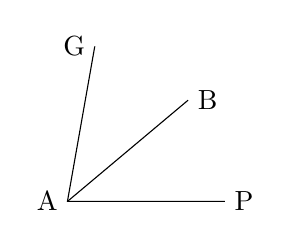
\begin{tikzpicture}
		\draw (0:2) coordinate [label=right:\pnt P] (P) 
			--(0,0) coordinate [label=left:\pnt A] (A)
			-- (80:2) coordinate [label=left:\pnt G] (G);
		\draw (A)--(40:2) coordinate [label=right:\pnt B] (B);
		\fillpoints {G,A,P,B}
		\mangle APB
		\mangleoffset ABG
		\end{tikzpicture}
		\begin{exparts}
		\item 54\degree
		\item 27\degree
		\end{exparts}
	\end{sol}
	\end{ex}
	
	\medskip
	\medskip
	
	\begin{ex}
	\e In the triangle below, use your ruler and protractor to determine whether \seg AM bisects \seg BC or \ang{BAC}.  Both? Neither?
	
	\begin{center}
	\begin{tikzpicture} [scale=0.8]
		\coordinate [label=below right:{\pnt M}]	(M) at (0,0);
		\coordinate [label=above left:{\pnt A}]	(A) at (160:3.8);
		\coordinate [label=right:{\pnt B}]		(B) at (33:4.1);
		\coordinate [label=below:{\pnt C}]		(C) at (213:4.1);
		\draw (A)--(B)--(C)--(A)--(M);
	\end{tikzpicture}
	\end{center}
	\begin{sol} 
	Only \seg BC 
	\end{sol}
	\end{ex}
	
	\begin{ex}
	\e Sketch a picture in which \segbis{KL}{PQ} 
	but $\seg KL\not\perp \seg PQ$. 
	Mark your diagram. 
	[Note: $\not\perp$ means \emph{not} perpendicular.] 
	\begin{sol}
	 \hspace*{\fill} \\
	\begin{tikzpicture}
	\draw (-1,0) coordinate [label=left:\pnt P] (P) -- (1,0) coordinate [label=right:\pnt Q] (Q);
	\coordinate (O) at (0,0);
	\draw (-1,1) coordinate [label=left:\pnt K] (K) -- (1,-1) coordinate [label=right:\pnt L] (L);
	\fillpoints {O,P,Q,K,L}
	\tick POOQ
	\end{tikzpicture}
	\end{sol}
	\end{ex}
	
	\medskip
	\newpage

	\begin{ex}
	\e Sketch a picture where \segperp {KL}{PQ} 
	but \seg KL does not bisect \seg PQ. 
	Mark your diagram.
	\begin{sol}
	 \hspace*{\fill} \\
	\begin{tikzpicture}
		\draw (0,0) coordinate [label=left:\pnt P] (P) 
			-- (3,0) coordinate [label=right:\pnt Q] (Q);
		\draw (1,.5) coordinate [label=right:\pnt K] (K) 
			-- (1,-.5) coordinate [label=right:\pnt L] (L);
		\coordinate (M) at (1,0);
		\fillpoints{D,P,O,F,M,K,L}
		\perpbox MQK
	\end{tikzpicture}
	\end{sol}
	\end{ex}
	
	\bigskip

	\begin{ex}
	\e Sketch a picture in which \seg KL is the perpendicular bisector of \seg PQ. 
	\begin{sol}
	 \hspace*{\fill} \\
	\begin{tikzpicture}
			\draw (0,0) coordinate [label=left:\pnt P] (P) 
				-- (3,0) coordinate [label=right:\pnt Q] (Q);
			\draw (1.5,.5) coordinate [label=right:\pnt K] (K) 
				-- (1.5,-.5) coordinate [label=right:\pnt L] (L);
			\coordinate (M) at (1.5,0);
			\fillpoints{P,Q,K,L,M}
			\tick PMMQ
			\perpbox MQK
	\end{tikzpicture}
	\end{sol}
	\end{ex}
	
	\bigskip

	\begin{ex}
	\e Sketch a picture that satisfies all of the following conditions.  Mark your diagram.
	\begin{itemize}
	\item \seg AB has \pnt E as a midpoint.
	\item \segperp{AB}{CD}, and \seg CD goes through \pnt B.
	\item \segcong{BD}{BE}
	\end{itemize}
	\begin{sol}
	 \hspace*{\fill} \\
		 \begin{tikzpicture}
		 \draw (0,0) coordinate [label=below:\pnt A] (A) 
			--(1,0) coordinate [label=below:\pnt E] (E) 
			-- (2,0) coordinate [label=right:\pnt B] (B);
		 \draw (2,.75) coordinate [label=right:\pnt C](C) 
			-- (2,-1) coordinate [label=right:\pnt D](D);
		 \perpbox BCE
		 \tick AEEB
		 \tick EBBD
		 \fillpoints {A,B,C,D,E}
		 \end{tikzpicture}
	\end{sol}
	\end{ex}
	
	\bigskip
	
	\begin{ex}
	\e Sketch a diagram in which \pnt B is on \seg CD. 
	If $\segl BC=2x+1$, $\segl BD=3x+2$, and $\segl CD=35$, find $x$ and \segl BD.
	\begin{sol}
	$x=6.4$, $\segl BD = 21.2$
	\end{sol}
	\end{ex}
	
	\bigskip
	\newpage

	\begin{ex}
	\e Sketch a diagram in which \seg AB and \seg CD are 
	perpendicular bisectors of each other, but $\seg AB \not\cong \seg CD$. [Note: $\not\cong$ means \emph{not} congruent.]
	\begin{sol}
	 \hspace*{\fill} \\
	\begin{tikzpicture}
			\draw (0,0) coordinate [label=left:\pnt A] (P) 
				-- (3,0) coordinate [label=right:\pnt B] (Q);
			\draw (1.5,.5) coordinate [label=right:\pnt C] (K) 
				-- (1.5,-.5) coordinate [label=right:\pnt D] (L);
			\coordinate (M) at (1.5,0);
			\fillpoints{P,Q,K,L,M}
			\tick PMMQ
			\ttick KMML
			\perpbox MQK
	\end{tikzpicture}
	\end{sol}
	\end{ex}
	
	\bigskip

	\begin{ex}
	\e Sketch a diagram in which \seg EF and \seg GH are
	perpendicular bisectors of each other, and \segcong {EF}{GH}.
	\begin{sol}
	 \hspace*{\fill} \\
	\begin{tikzpicture}
			\draw (0,0) coordinate [label=left:\pnt A] (P) 
				-- (2,0) coordinate [label=right:\pnt B] (Q);
			\draw (1,1) coordinate [label=right:\pnt C] (K) 
				-- (1,-1) coordinate [label=right:\pnt D] (L);
			\coordinate (M) at (1,0);
			\fillpoints{P,Q,K,L,M}
			\tick PMMQ
			\tick KMML
			\perpbox MQK
	\end{tikzpicture}
	\end{sol}
	\end{ex}
	
	\bigskip

	\begin{ex}
	\e Gerry Geometry wants to build a house that is the same distance
	from Krispy Kreme (\pnt K) as it is from WaWa (\pnt W).
	Place dots at at least three different places he could live.
	What do the three points have in common?\\

	\begin{tikzpicture}
		\draw (0,0) coordinate [label=left:\pnt K] (K)
			-- (4,1) coordinate [label=right:\pnt W] (W);
		\fillpoints {K,W}
	\end{tikzpicture}
	
	\begin{sol} All the points are on the perpendicular bisector of \seg KW \end{sol}
	\end{ex}
	
	\bigskip

	\begin{ex}
	\e If \segperp {XY}{PO}, does one of the segments 
	have to be the perpendicular bisector of the other? Explain.
	\begin{sol}
	No. 
	It is possible for two segments to be perpendicular but neither one bisects the other.
	\end{sol}
	\end{ex}
	
	\bigskip
	\newpage
	
	\begin{ex}
	Sketch and describe the locus of points in a plane, equidistant from \pnt M and \pnt N.  \textbf{Advanced Challenge:}  Describe how you would \emph{construct} it.\\
	
	\begin{center}
	\begin{tikzpicture}
		\coordinate [label=right:{\pnt M}]	(M) at (0,0);
		\coordinate [label=right:{\pnt N}]	(N) at (0,4);
		
		\fillpoints {M,N}
	\end{tikzpicture}	
	\end{center}
	
	\begin{sol}
	It is a sketch of the perpendicular bisector of \seg MN.
	\end{sol}
	\end{ex}
	
	
	
\end{exercises}

%------------------------------------------------------------------------------------
			\section{Advanced:  Constructing Perpendiculars and Bisectors}
%------------------------------------------------------------------------------------

Reminder:  Any line can be drawn, but a ``particular'' line must have two points to define it!  Please \emph{do not} ``eyeball'' it.  Placing of a compass pin must be at a particular point, \emph{not} an eyeballed placement.  Remember:  particular points are found at the intersection of two lines or arcs.

\subsection{Constructing the Perpendicular Bisector of a Segment}

The goal is to construct the perpendicular bisector of a given segment.  Segment \seg AB is below. \q Construct the perpendicular bisector of \seg AB.

\begin{enumerate}
\item Place the pin on one of the endpoints of the segment and open it up to a little more than halfway to the other endpoint.
\item Make an arc so that the ends of it are closer to the pin than to the other endpoint.
\item Without changing the size of the compass, make another similar arc with the pin on the other endpoint.
\item Mark the two points of intersection of the two arcs.  Use your straight edge to make a line that passes through both of those points.  Mark your drawing.
\end{enumerate}

\vspace{1cm}

\begin{center}
\begin{tikzpicture}

	\coordinate [label=below:$A$] (A) at (0,0);
	\coordinate [label=below:$B$] (B) at (5,0);	
	\draw (B)--(A);	
	\fillpoints {B,A}
	
\end{tikzpicture}
\end{center}

\vspace{0.5cm}

\subsection{Drop a Perpendicular}
The goal is to construct a line perpendicular to a given line, through a given point.  Segment \seg GH is below.\q Construct \emph{two} perpendicular lines: one through $E$, a point on the segment, and one through $D$, a point not on the segment.\\

\noindent For constructing through point \pnt E:
\begin{enumerate}
\item Place the pin on E and make two markings equidistant from \pnt E on \seg GH.
\item Using these two new points, follow the steps for making a perpendicular bisector.
\end{enumerate}
For constructing through point \pnt D:
\begin{enumerate}
\item Place the pin on \pnt D and open up the compass to a little past \seg GH.
\item Make an arc that intersects \seg GH at two points.
\item Using these two points of intersection, follow the steps for making a perpendicular bisector. 
\end{enumerate}

\vspace{0.75cm}

\begin{center}
\begin{tikzpicture}

	\coordinate [label=below:$G$] (G) at (0,0);
	\coordinate [label=below:$H$] (H) at (9,0);	
	\coordinate [label=below:$E$] (E) at (2,0);
	\coordinate [label=right:$D$] (D) at (6,3);
	\draw (G)--(H);	
	\fillpoints {G,H,E,D}
	
\end{tikzpicture}
\end{center}

\vspace{2cm}

\subsection{Constructing an Angle Bisector}
The goal is a to construct a ray that bisects a given angle. \q $\angle DEF$ is pictured below, construct angle bisector $\overrightarrow{EG}$.

\begin{enumerate}
\item Open your compass up to any size.  Place the pin on the vertex and make an arc that intersects both sides of the angle.
\item Place the pin at one of the intersection points of the sides and open it to over half way to the other intersection point. (you might be able to keep it the same as the original size).
\item With the pin on the intersection point, make an arc on the other side of original arc from the vertex.  Make sure it crosses the anticipated angle bisector.
\item Without changing the size of the compass, make a similar arc from the other point of intersection. 
\item Draw a ray from the vertex through the intersection point of the two arcs.  Mark your drawing.
\end{enumerate}

	\begin{center}
	\begin{tikzpicture}
		\coordinate [label=left:{$E$}]		(X) at (0,0);
		\coordinate [label=below:{$D$}] 	(Y) at (0:4);
		\coordinate [label=left:{$F$}]		(Z) at (60:4);
		\raydraw{X}{Z}
		\raydraw{X}{Y}
		\fillpoints{Y,X,Z}
	\end{tikzpicture}
	\end{center}

\begin{exercises}
	\begin{ex}
	Construct the perpendicular bisector of $\overline{YZ}$.\\

\vspace{0.5cm}

\begin{center}
\begin{tikzpicture}

	\coordinate [label=below:$Y$] (G) at (0,0);
	\coordinate [label=below:$Z$] (H) at (5,1);	
	\draw (G)--(H);	
	\fillpoints {G,H}
	
\end{tikzpicture}
\end{center}

	\begin{sol}
	Construction
	\end{sol}
	\end{ex}
	
	\newpage
	
	\begin{ex}
	Construct the midpoint of $\overline{PQ}$. Label the midpoint $N$.

\vspace{0.5cm}

\begin{center}
\begin{tikzpicture}

	\coordinate [label=below:$P$] (G) at (0,2);
	\coordinate [label=below:$Q$] (H) at (5,0);	
	\draw (G)--(H);	
	\fillpoints {G,H}
	
\end{tikzpicture}
\end{center}
	\begin{sol}
	Construction
	\end{sol}
	\end{ex}
	
	\begin{ex}
	Construct perpendicular bisectors that divide $\overline{EF}$ into four congruent segments.

\vspace{1.5cm}

\begin{center}
\begin{tikzpicture}

	\coordinate [label=below:$E$] (G) at (0,0);
	\coordinate [label=below:$F$] (H) at (8,0);	
	\draw (G)--(H);	
	\fillpoints {G,H}
	
\end{tikzpicture}
\end{center}

\vspace{1.5cm}
	\begin{sol}
	Construction
	\end{sol}
	\end{ex}
	
	\begin{ex}
	Using the previous two constructions, construct a segment whose length is $\frac{1}{2}PQ+\frac{3}{4}EF$.
	\begin{sol}
	Construction
	\end{sol}
	\end{ex}
	
	\bigskip
	
	\begin{ex}
	Construct a line perpendicular to $\overline{SM}$ through $S$.

\vspace{1cm}

\begin{center}
\begin{tikzpicture}

	\coordinate [label=below:$S$] (G) at (0,0);
	\coordinate [label=below:$M$] (E) at (6,2);

	\draw (G)--(E);	
	\fillpoints {G,E}
	
\end{tikzpicture}
\end{center}

\vspace{1cm}
	\begin{sol}
	Construction
	\end{sol}
	\end{ex}
	
	\begin{ex}
	Construct $\angle KLM$ that has a measure of $45^\circ$.
	\begin{sol}
	Construction
	\end{sol}
	\end{ex}
	
	\bigskip
	\medskip
	
	\begin{ex}
	Construct a perpendicular line from \pnt A to \lin BC.  Then use a ruler to measure the distance from \pnt A to \lin BC.\\  

\begin{center}
\begin{tikzpicture}

	\coordinate [label=above:$A$] (A) at (5,2.5);
	\coordinate [label=below:$B$] (G) at (0,0);
	\coordinate [label=below:$C$] (H) at (8,0);	
	\draw [triangle 45-triangle 45] (-1,0)--(9,0);	
	\fillpoints {A,G,H}
	
\end{tikzpicture}
\end{center}

	\begin{sol}
	Construction, length is $2.5~cm$
	\end{sol}
	\end{ex}
\end{exercises}	
		
\section{Mixed Review}	

This book contains sections of review problems that combine terms, concepts and skills across multiple sections and can cross chapters as well.  These sections will help you to consolidate the information and prepare for quizzes and tests.

\begin{exercises}
	\begin{ex}
	\e Sketch a diagram in which \ray OG bisects \ang{MON}. 
	Given that $\angm{MOG}=38\degree$ and $\angm{NOG}=6y\degree$, find $y$.
	\begin{sol} $\frac{19}{3}$ \end{sol}
	\end{ex}
	
	\medskip
	
	\begin{ex}
	\e In the diagram below, explain why \segcong{BA}{BC}.
	
	\begin{tikzpicture}
		\draw (0,0) coordinate [label=below:\pnt A] (a)
			-- (2,0) coordinate [label=below:\pnt D] (d)
			-- (4,0) coordinate [label=below:\pnt C] (c)
			-- (2,1) coordinate [label=above:\pnt B] (b)
			--cycle;
		\draw (b)--(d);
		\perpbox dcb
		\tick addc
	\end{tikzpicture}
	\begin{sol}
		Since  \seg BD is the perpendicular bisector of
		 \seg AC, then  \pnt B is the same distance
		from  \pnt A and  \pnt C. Thus,  \segcong {AB}{AC}.
	\end{sol}
	\end{ex}
	
	\smallskip
	
	\begin{ex}
	\e Consider the diagram with the following information. 

\begin{center}
\begin{tikzpicture}

	\coordinate [label=below:{$T$}]	(Q)	at (0,0);
	\coordinate [label=below:{$Z$}]	(R)	at (3.2,0.8);
	\coordinate [label=below:{$A$}]	(S)	at (7.5,1.875);
	\coordinate [label=below:{$G$}]	(T)	at (12,3);
	\coordinate [label=above:{$M$}]	(O)	at (2,2);
	\coordinate [label=above:{$W$}]	(P)	at (3,3);
	\coordinate [label=above:{$Y$}]	(U)	at (7.5,4);
	
	\draw (Q)--(R)--(S)--(T);
	\draw (Q)--(O)--(P)--(S);
	\draw (O)--(R);
	\draw (S)--(U);
	
	\foreach \point in {O,P,Q,R,S,T,U} \fill (\point) circle (1.5pt);

\end{tikzpicture}
\end{center}


	\begin{multicols}{2}
	\begin{exparts}
		\item Is $G$ on $\overleftrightarrow{TA}$?
	\vfill
		\item Is $G$ on $\overrightarrow{TA}$?
	\vfill
		\item Is $G$ on $\overline{TA}$?
	\vfill
		\item Is $G$ on $\overrightarrow{AT}$?
	\vfill
		\item Name three points that are collinear?
	\vfill
		\item Measure $WT$.
	\columnbreak
%	\vspace{1.25cm}
		\item Measure $\angle MZA$.
	\vfill
		\item Classify $\angle MZA$ as acute, right, or obtuse.
	\vfill
		\item Give another name for $\overrightarrow{TZ}$.
	\vfill
		\item Name an angle that looks acute.
	\vfill
		\item Name the vertex of $\angle YAG$.
	\vfill
		\item Name a line containing point $T$.
	\vfill
%	\columnbreak
	\end{exparts}
	\end{multicols}
	\begin{sol}
	\begin{exparts}
	\item Yes
	\item Yes
	\item No
	\item No
	\item Z,A and G (other poss.)
	\item 4.1 cm or 1$\dfrac{5}{8}$ in
	\item $122\degree$
	\item obtuse
	\item \ray TA
	\item $\angle WAY$ (other poss.)
	\item A
	\item \lin TW (other poss.)
	\end{exparts}
	\end{sol}
	\end{ex}
	
	\begin{ex}
	\e Sketch a diagram below that satisfies all of the following conditions. Mark your diagram.
	\begin{exparts}
		\item $\angle MNO = 120^\circ$
		\item $\angle MNP$ is a straight angle
		\item $\overline{MN} \cong \overline{NP}$
	\end{exparts}
	\begin{sol}
	 \hspace*{\fill} \\
	\begin{tikzpicture} [font=\scriptsize]
		\coordinate [label=below:{\pnt N}] 		(N) at (0,0);
		\coordinate [label=below:{\pnt M}] 		(M) at (1,0);
		\coordinate [label=right:{\pnt O}] 		(O) at (120:1);
		\coordinate [label=below:{\pnt P}] 		(P) at (-1,0);	
		\coordinate [label=above right:{$120\degree$}] 		(N) at (0,0);	
		\linedraw MP
		\raydraw NO
		\fillpoints{N,M,O,P}
		\ttick MNNP
	\end{tikzpicture}
	\end{sol}
	\end{ex}
	\medskip
	
\begin{ex} \e Consider \cir O.  Solve for $x$.	

\begin{center}
\begin{tikzpicture} 
	\coordinate [label=left:{$O$}]	(O)	at (0,0);
	\coordinate [label=above left:{}]	(R)	at (30:1.5);
	\coordinate [label=above right:{}]	(S)	at (-40:1.5);
	
	\draw (O) circle (1.5cm);
	\draw (O)--(R) node [pos=0.5, above left] {$x$}--(S) node [pos=0.5, left] {7}--(O) node[pos=0.5, below left] {6};
	
	\foreach \point in {O} \fill (\point) circle (1.5pt);

\end{tikzpicture}
\end{center}
\begin{sol}
$x=6$
\end{sol}
\end{ex}
	


\begin{ex}
	You will sketch a diagram in Part (a) and use it to answer Parts (b - e).
	\begin{exparts}
	\item \e Sketch and mark a diagram in which $\overline{AB}$ is perpendicular to $\overline{PQ}$ at point $X$, but does not bisect $\overline{PQ}$. 
	\medskip
	\item \e Name 3 collinear points.
	\smallskip
	\item \e Name 3 non-collinear points.
	\smallskip
	\item If m$\angle QXB$ = $14a^\circ$, find $a$. 
	\medskip
	\item If $AX=20$, $XB=z+6$, and $AB=3z$, find $z$. \vfill
	\end{exparts}
	\begin{sol}
	\begin{exparts}
	\item \hspace*{\fill} \\
	\begin{tikzpicture} [font=\scriptsize]
		\coordinate [label=below left:{\pnt X}] 		(X) at (0,0);
		\coordinate [label=below:{\pnt A}] 		(A) at (-1.5,0);
		\coordinate [label=below:{\pnt B}] 		(B) at (1.4,0);
		\coordinate [label=left:{\pnt P}] 		(P) at (0,1);	
		\coordinate [label=right:{\pnt Q}] 		(Q) at (0,-1.5);
		\draw (A)--(B);
		\draw (P)--(Q);
		\fillpoints{X,A,B,P,Q}
		\perpbox XBP
	\end{tikzpicture}
	\item A,X,B or P,X,Q
	\item A,X,P and others
	\item $a = \frac{45}{7}$
	\item $z = 13$
	\end{exparts}
	\end{sol}
	\end{ex}
	\medskip
	
	\begin{ex}
	\e Sketch a diagram that satisfies the following conditions. Be sure to mark your diagram appropriately.
	\begin{exparts}
	\item $\overline{AC}\perp\overline{CF}$.
	\item $D$ is the midpoint of $\overline{CF}$.
	\item Draw \seg AD
	\item $\overrightarrow{DZ}$ bisects $\angle ADF$.
	\end{exparts}
	\begin{sol}
	 \hspace*{\fill} \\
	\begin{tikzpicture} [font=\scriptsize]
		\coordinate [label=below:{\pnt D}] 		(D) at (0,0);
		\coordinate [label=below:{\pnt F}] 		(F) at (-1,0);
		\coordinate [label=below:{\pnt C}] 		(C) at (1,0);
		\coordinate [label=right:{\pnt A}] 		(A) at (1,2);	
		\coordinate [label=right:{\pnt Z}] 		(Z) at (122:1);	
		\draw (F)--(C)--(A)--(D);
		\raydraw DZ
		\fillpoints{D,F,C,A,Z}
		\ttick FDDC
		\mmangle DAZ
		\mmangleoffset DZF
		\perpbox CAF
	\end{tikzpicture}
	\end{sol}
	\end{ex}
	\medskip
	
	\begin{ex}
	You will sketch a diagram in Part (a) and use it to answer Part (b).
	\begin{exparts}
	\item \e Sketch and mark a diagram in which $\overrightarrow{PQ}$ bisects $\angle SPR$. 	
	
	\item If m$\angle SPQ=(x+25)^\circ$ and m$\angle SPR = (6x-2)^\circ$, find $x$ and m$\angle QPR$.
	\end{exparts}
	\begin{sol}
	\begin{exparts}
	\item \hspace*{\fill} \\
	\begin{tikzpicture} [font=\scriptsize]
		\coordinate [label=below:{\pnt P}] 		(P) at (0,0);
		\coordinate [label=below:{\pnt R}] 		(R) at (1,0);
		\coordinate [label=below:{\pnt Q}] 		(Q) at (35:1);
		\coordinate [label=left:{\pnt S}] 		(S) at (70:1);	
		\raydraw PR
		\raydraw PQ
		\raydraw PS
		\fillpoints{P,R,Q,S}
		\mmangle PRQ
		\mmangleoffset PQS
	\end{tikzpicture}
	\item $x = 13$, $\angm {QPR}=38\degree$
	\end{exparts}
	\end{sol}
	\end{ex}
	\bigskip
	\medskip
	
	\begin{ex} Consider $\odot Q$.  Diagram not necessarily drawn to scale, do not use measuring tools for this problem.

\begin{exparts}
\item Solve for $a$.

\begin{flushright}
\begin{tikzpicture} [scale=0.7]
	\coordinate [label=below:{$Q$}]	(Q)	at (0,0);
	\coordinate [label=above left:{$R$}]	(R)	at (120:3);
	\coordinate [label=above right:{$S$}]	(S)	at (40:3);
	
	\draw (Q) circle (3cm);
	\draw (Q)--(R) node [pos=0.5, sloped, below] {\small{$4a+1$}}--(S) node [pos=0.5, sloped, above] {\small{$6a-3$}}--(Q) node[pos=0.5, sloped, below] {\small{$7a-13$}};
	
	\foreach \point in {Q,R,S} \fill (\point) circle (1.5pt);

\end{tikzpicture}
\end{flushright}

\item Give the length of \seg RS.
\end{exparts}

\begin{sol}
$a=\frac{14}{3}$, \seg RS = 25
\end{sol}
\end{ex}
\smallskip	
	
\end{exercises}

\section{Angle Relationships}
\subsection{Complement/complementary}
\textbf{Complementary angles} are two angles whose measures sum to 90\degree.  When you see a right angle in a geometry diagram, you can sometimes find complementary angles lurking around.

In the diagram below, \ang{EGD} and \ang{DGR} are complementary. 
You can say that they are \textbf{complements} of each other.
\q If the m\ang{DGR} = 20\degree, give the m\ang{EGD}.

	\begin{center}
	\begin{tikzpicture}
		\coordinate [label=left:{\pnt E}]		(E) at (1,0);
		\coordinate [label=right:{\pnt G}]	(G) at (5,0);
		\coordinate [label=below:{\pnt R}]	(R) at (5,-2);
		\coordinate [label=below:{\pnt D}]	(D) at (4,-2);
		\draw (E)--(G)--(R);
		\draw (G)--(D);
		\perpbox {G}{E}{R}
	\end{tikzpicture}
	\end{center}
	
\q If the m\ang{DGR} = x\degree, give the m\ang{EGD}.	
	
\noindent You do not need a diagram to work with complementary angles. 

\q What is the complement of a $40\degree$ angle?

\subsection{Linear pair}
One type of angle relationship appears quite frequently in geometry. 
When \emph{two} non-overlapping angles 
are \emph{adjacent}\footnote{The word \emph{adjacent} 
has a complicated geometry definition. 
If you think of adjacent as meaning ``next to'', you will have the right idea.}, 
share the same vertex, and add up to a straight angle, 
they are said to form a \textbf{linear pair}. 
Visually, linear pairs look like a ``line'' divided into two angles.

	\begin{center}
	\begin{tikzpicture}
		\coordinate [label=below:{\pnt A}]	(A) at (-2,0);
		\coordinate [label=below:{\pnt C}]	(C) at (0,0);
		\coordinate [label=below:{\pnt B}]	(B) at (2,0);
		\coordinate [label=above:{\pnt D}]	(D) at (1,1.5);
		\draw (A)--(B);
		\draw (C)--(D);
	\end{tikzpicture}
	\end{center}

In the diagram above, \ang{BCD} and \ang{DCA} form a linear pair. \q What is the sum of the measures of these two angles?

\paragraph{Course Convention}  Angles are numbered \ang 1, \ang 2, etc. to make a problem easier to write and communicate about.  It is important to remember that when an number carries degrees (\degree), it is a measure.  When angles are numbered without degrees, they are numbered for your convenience.  (Reminder:  a capital letter at an angle refers to the point of intersection.)\\

Linear pairs can be challenging to see when the diagrams get more complicated. 
\q Name at least one linear pair in each diagram below. 

	\begin{tikzpicture}
		\coordinate [label={[shift={(.3,-.1)}] \scriptsize 1}] 		(A) at (0,0);
		\coordinate [label={[shift={(-.4,-.1)}] \scriptsize 2}]		(B) at (3,0);
		\coordinate [label={[shift={(.05,-.55)}] \scriptsize 3},
					label={[shift={(.2,-.2)}] \scriptsize 4}]	(C) at (1,2);
		\coordinate 									(D) at (1.5,3);
		\draw (D)--(A)--(B)--(C);
	\end{tikzpicture}
	\hfill
	\begin{tikzpicture}
		\coordinate [label={[shift={(-.2,.1)}] \scriptsize 5},
					label={[shift={(.1,.05)}] \scriptsize 6},
					label=0:{\scriptsize 7},
					label=below left:\pnt O](O) at (0,0);
		\coordinate [label=left:\pnt M] (M) at (140:2);
		\coordinate [label=right:\pnt N] (N) at (-40:2);
		\coordinate [label=above:\pnt P] (P) at (100:2);
		\coordinate [label=above:\pnt Q] (Q) at (50:2);
		\draw(M)--(O)--(N);
		\draw (P)--(O)--(Q);
	\end{tikzpicture}
	\hfill
	\begin{tikzpicture}
		\coordinate [label={[shift={(.05,.3)}] \scriptsize 8},
					label={[shift={(.35,.25)}] \scriptsize 9},
					label={[shift={(-.15,-.05)}] \scriptsize 10},
					label={[shift={(.3,-.1)}] \scriptsize 11}]
				(X) at (0,.3);
		\coordinate [label={[shift={(-.1,0)}] \scriptsize 12},
					label={[shift={(.35,.05)}] \scriptsize 13},
					label={[shift={(-.25,-.35)}] \scriptsize 14},
					label={[shift={(.2,-.3)}] \scriptsize 15}]
				(Y) at (-.5,-1);
		
		\draw ($(X)!1cm!180:(Y)$)--($(Y)!.5cm!180:(X)$);
		\draw (-1.5,1)--(1,.5);
		\draw (-1.5,-1)--(1,-.75);
	\end{tikzpicture}

\noindent \q The measures of the angles of a linear pair add up to 180\degree. (Why?)
\medskip

\subsection{Supplement/supplementary}

\textbf{Supplementary angles} are two angles whose measures sum to 180\degree.

In the diagram below, \ang{ACE} and \ang{ECB} are supplementary.
	\begin{center}
	\begin{tikzpicture}
		\coordinate [label=below:\pnt C] (C) at (0,0);
		\coordinate [label=above:\pnt A] (A) at (160:2);
		\coordinate [label=below:\pnt B] (B) at (-20:3);
		\coordinate [label=below:\pnt D] (D) at (220:2);
		\coordinate [label=above:\pnt E] (E) at (40:3);
		\draw (A)--(B);
		\draw (D)--(E);
	\end{tikzpicture}
	\end{center}
\noindent \q Name another pair of supplementary angles in the diagram above.

\newpage

Supplementary angles need not be adjacent. 
The angles below are supplementary even though they are not ``next to'' each other.\\
	\begin{center}
	\begin{tikzpicture}
		\coordinate [label=below left:\pnt A,label={[shift={(.25,0)}] 
			\scriptsize 140\degree}] (A) at (0,0);
		\coordinate [label=below left:\pnt B,label={[shift={(.6,-.08)}] 
			\scriptsize 40\degree}] (B) at (5,0);
		\raydraw{A}{2,0}
		\raydraw{A}{140:2}
		\raydraw{B}{7,0}
		\raydraw{B}{{5+2*cos(40)},{2*sin(40)}}
	\end{tikzpicture}
	\end{center}
	
	\medskip
	
\subsection{Vertical angles}

When two lines intersect, they intersect at a single point making an \emph{X}.\\

The angles across from each other are called \textbf{vertical angles} 
(even if they are not actually ``vertical'' in the picture).\\

In the diagram below, \ang{CEB} and \ang{DEA} are vertical angles.

	\begin{center}
	\begin{tikzpicture}
		\coordinate [label=above:\pnt E] (E) at (0,0);
		\coordinate [label=left:\pnt C] (C) at (190:2);
		\coordinate [label=right:\pnt D] (D) at (10:2);
		\coordinate [label=right:\pnt A] (A) at (320:2);
		\coordinate [label=left:\pnt B] (B) at (140:2);
		\draw [latex-latex] (C)--(D);
		\draw [latex-latex] (A)--(B);
	\end{tikzpicture}
	\end{center}
	
\noindent \q Name another pair of vertical angles in the picture above. 
\vspace{1.0cm}

\noindent \q Give the name of the relationship between \ang{CEA} and \ang{DEA}. 
\vspace{1.0cm}

\noindent \q Can you give the sum of m\ang{CEA} and m\ang{DEA}. 
\medskip

\newpage

\subsection{Exploration: Vertical angles}

Use the numbered angles in the diagram below:

\begin{enumerate}
\item List all of the pairs of vertical angles.
\item List all of the linear pairs.
\smallskip
 

	\begin{center}
	\begin{tikzpicture}
		\coordinate [label=below:] (F) at (0,0);
		\coordinate [label=left:] (G) at (170:3.5);
		\coordinate [label=right:] (J) at (-10:4);
		\coordinate [label=left:] (A) at (205:3.75);
		\coordinate [label=right:] (C) at (25:4.25);
		\coordinate [label=right:3] (X) at (8:0.5);
		\coordinate [label=above:2] (Y) at (95:0.1);
		\coordinate [label=left:1] (Z) at (188:0.5);
		\coordinate [label=below:4] (W) at (275:0.1);
		\draw [latex-latex] (G)--(J);
		\draw [latex-latex] (A)--(C);
	\end{tikzpicture}
	\end{center}
	
\item Use a protractor to measure all the angles in the diagram and fill them in on your diagram.	

\item What do we know about the measures of all linear pairs?
\medskip

\item Do these angle measures make sense?  Explain why or why not?
\bigskip

\item Write a conjecture about any pair of vertical angles?  
\medskip
\end{enumerate}

\noindent \aq Write a sentence or two to justify this conjecture?
\bigskip
\newpage

\noindent These two relationships are present whenever two lines intersect\ldots
\begin{tcolorbox}
(a) \textbf{Linear Pair} and (b) \textbf{Vertical Angles (theorem)} 
\begin{center}
\begin{tikzpicture}

	\coordinate[label=below:{}]				(A)	at	(180:1.5);
	\coordinate[label=below:{}]				(B)	at	(0:1.5);
	\coordinate[label=below:{}]				(C)	at	(110:1.5);
	\coordinate[label=below:{}]				(D)	at	(290:1.5);
	\coordinate[label=below:{(a) Linear pairs are always supplementary.}]				(E)	at	(1.5,-1.75);
	\coordinate[label=below:{(b) Any pair of vertical angles are congruent.}]				(F)	at	(1.5,-2.25);
	\node [right] at (15:3) {Linear pair with \ang 1};
		\draw [->] (18:2.9) to [bend right] (0.2,0.2);
	\node [right] at (-15:3) {Vertical angles with \ang 1};
		\draw [->] (-18:2.9) to [bend left] (0.3,-0.2);	
	
	
	\draw [latex-latex, thick] (A)--(B) node [pos=0.35, above] {1};
	\draw [latex-latex, thick] (C)--(D);
		
\end{tikzpicture}
\end{center}
\end{tcolorbox}
	
\begin{exercises}
	\begin{ex}
	\e Make note cards for:  \textbf{Complementary angles}, \textbf{Linear Pair}, \textbf{Supplementary angles} and \textbf{Vertical Angles}.  
	\begin{sol}
	Note cards
	\end{sol}
	\end{ex}
		\begin{ex}
		\e Use the diagram below to answer the questions that follow.

	\begin{center}
	\begin{tikzpicture}
		\coordinate [label=below right:\pnt C,
					label={[shift={(.55,.02)}] \scriptsize 40\degree},
					label={[shift={(-.7,-.22)}] \scriptsize 30\degree}] 
				(C) at (0,0);
		\coordinate [label=left:\pnt A] (A) at (190:1.5);
		\coordinate [label=right:\pnt B] (B) at (10:1.5);
		\coordinate [label=above:\pnt D] (D) at (100:1.5);
		\coordinate [label=below:\pnt E] (E) at (280:1);
		\coordinate [label=above left:\pnt F] (F) at (160:1.5);
		\coordinate [label=above right:\pnt G] (G) at (50:1.5);
		\draw (A)--(B);
		\draw (D)--(E);
		\draw (F)--(C)--(G);
		\perpbox{C}{B}{D}
	\end{tikzpicture}
	\end{center}
	
	\begin{exparts}
	\begin{multicols}{2}
%	\itemsep = \smallskipamount
			\item Find \angm{DCB}.			
			\item Find \angm {GCB}. 			
			\item Find \angm {DCG}.			
			\item Find \angm {DCF}.
			\item Find \angm {BCF}.			
			\item Find \angm {BCE}.			
			\item Find \angm {DCE}.			
			\item Name a complement of \ang{FCA}.
			\item Name a supplement of \ang {FCA}. 
			\item How are \ang {DCG} and \ang {ECG} related?
	\end{multicols}
	\end{exparts}
	\begin{sol}
	\hspace*{\fill}
	\begin{exparts}
		\item 90\degree
		\item 40\degree
		\item 50\degree
		\item 60\degree
		\item 150\degree
		\item 90\degree
		\item 180\degree
		\item \ang{FCD}
		\item \ang{FCB}
		\item They form a linear pair.
	\end{exparts}
	\end{sol}
	\end{ex}
	
	\begin{ex}
\e In each of the diagrams below, 
one angle measurement is given. 
Find the other three angles.

(a) \hspace*{\fill} (b) \hspace*{\fill}

	\begin{tikzpicture}
		\coordinate [label={[shift={(.25,-.6)}] \pnt Z},
					label={[shift={(-.35,.1)}] 100\degree}] (X) at (0,0);
		\coordinate [label=left:\pnt W] (W) at (170:1.75);
		\coordinate [label=right:\pnt A] (A) at (-10:2.2);
		\coordinate [label=250:\pnt V] (V) at (250:1.5);
		\coordinate [label=70:\pnt Y] (Y) at (70:1.25);
		\draw [latex-latex] (W)--(A);
		\draw [latex-latex] (V)--(Y);
	\end{tikzpicture}
	\hspace*{\fill}
	\begin{tikzpicture}
		\coordinate [label=below:\pnt P,
				label={[shift={(-.8,-.15)}] 40\degree}] (P) at (0,0);
		\coordinate [label=above left:\pnt Q] (Q) at (150:2);
		\coordinate [label=below right:\pnt R] (R) at (-30:2);
		\coordinate [label=left:\pnt S] (S) at (190:1.75);
		\coordinate [label=right:\pnt T] (T) at (10:2.25);
		\draw [latex-latex] (Q)--(R);
		\draw [latex-latex] (S)--(T);
	\end{tikzpicture}
	\hspace*{\fill}
\begin{sol}
\hspace*{\fill}
\begin{exparts}
\item $ \angm {VZA}=100\degree$, $ \angm {YZA}=\angm{WZV}=80\degree$
\item $ \angm {TPR}=40\degree$, $ \angm {QPT}=\angm{SPR}=140\degree$
\end{exparts}
\end{sol}
\end{ex}	
	
	
	\begin{ex}
	\e Solve for $x$ in the diagram below.
	\begin{center}
	\begin{tikzpicture}
		\coordinate [label=below:\pnt C,
					label={[shift={(.85,-.05)}] \scriptsize $(3x+4)\degree$},
					label={[shift={(-.7,-.05)}] \scriptsize $(2x+6)\degree$}] 
				(C) at (0,0);
		\coordinate [label=left:\pnt A] (A) at (180:2);
		\coordinate [label=right:\pnt B] (B) at (0:2);
		\coordinate [label=above:\pnt D] (D) at (80:2);
		\draw (A)--(B);
		\draw (D)--(C);
	\end{tikzpicture}
	\end{center}
	\begin{sol} 34 \end{sol}
	\end{ex}
	
	\begin{ex}
	Find the measure of an angle that is 10\degree \ greater than its linear pair. 
	\begin{sol}
	95\degree
	\end{sol}
	\end{ex}
	
	\medskip
	
	\begin{ex}
	Find the measure of an angle that is twice as large as its complement.
	\begin{sol} 60\degree \end{sol}
	\end{ex}
	
	\medskip

	\begin{ex}
	\e Are the angles that form a linear pair always supplementary? 
	Explain.
	\begin{sol}
	Yes, the angles forming a linear pair add up to a straight angle, which is 180\degree .
	\end{sol}
	\end{ex}
	
	\smallskip
	
	\begin{ex}
	\e Do supplementary angles always form a linear pair? 
	Explain.
	\begin{sol} No, supplementary angles need not be right next to each other.\end{sol}
	\end{ex}
	
	\smallskip
	\newpage
	
	\begin{ex}
	An angle is 15\degree \ more than twice its complement. 
	Find the measure of the angle.
	\begin{sol} 65\degree \end{sol}
	\end{ex}
	\bigskip
		
\begin{ex}
Use the diagram below to answer the following questions.
	\begin{center}
	\begin{tikzpicture}
		\coordinate [label=below:\pnt K] (K) at (0,0);
		\coordinate [label=above left:\pnt F] (F) at (167:2);
		\coordinate [label=above right:\pnt G] (G) at (13:2);
		\coordinate [label=left:\pnt H] (H) at (193:2);
		\coordinate [label=right:\pnt J] (J) at (-13:2);
		\draw [latex-latex] (G)--(H);
		\draw [latex-latex] (F)--(J);
	\end{tikzpicture}
	\end{center}
	\begin{exparts}
	
		\item \e Solve for $a$, given $\angm{FKH}=(2a+5)\degree$ and
		$\angm{GKJ}=(10a-75)\degree$. 
		\medskip
	
		\item Find \angm{JKG} and \angm{JKH}.
		\medskip
	\end{exparts}
\begin{sol}
\hspace*{\fill}
\begin{exparts}
\item 10
\item 25, 155
\end{exparts}
\end{sol}
\end{ex}

\begin{ex}
In a sentence or two, write down your reasoning as to why your Vertical Angles Conjecture is true.
\begin{sol} Answers may vary.  Vertical Angles are supplements to the same angle. \end{sol}
\end{ex}

\medskip

\begin{ex}
Sketch a picture in which \seg BD and \seg CE intersect at \pnt A. 
Let $\angm{BAC}=(2x+3y)\degree$,
$\angm{BAE}=(10y+4)\degree$,
and $\angm{EAD}=(6x-4)\degree$.
Find $x$ and $y$.
\begin{sol}
$x=10$, $y=12$
\end{sol}
\end{ex}

\vspace{6cm}

\end{exercises}
\newpage


\section{Parallel (lines)}
\subsection{Definition of parallel}
In a plane (two dimensions), lines that do not intersect are called \textbf{parallel}.

The symbol for ``is parallel to'' is $\parallel$.

In a diagram, identical arrowheads are used to show that two lines are parallel.\\ 
**If you do not see the arrowheads, you should not assume the lines are parallel.

In the picture below, $\seg AB\parallel\seg CD$.

	\begin{center}	
	\begin{tikzpicture}
		\coordinate [label=below left:\pnt A] (A) at (0,0);
		\coordinate [label=right:\pnt B] (B) at (3,1.5);
		\coordinate [label=below left:\pnt C] (C) at (2,-1);
		\coordinate [label=above right:\pnt D] (D) at (4,0);
		\draw (A)--(B);
		\draw (C)--(D);
		\parrow{A}{B}{C}{D}
	\end{tikzpicture}
	\end{center}

In \emph{three dimensions}, it is possible for lines to not intersect or be parallel. 
Such lines are called \textbf{skew}. 
Skew lines are noncoplanar lines.

\q In our classroom, identify the following: parallel lines, perpendicular lines, skew lines.
\medskip

\q Explain why you can not sketch skew lines in the margin.
\smallskip

\noindent Here is a variation of another one of Euclid's 5 axioms\ldots
\begin{tcolorbox}
\textbf{Parallel postulate (alternative statement: Playfair's Axiom)} \\
\begin{center}
\begin{tikzpicture}

	\coordinate[label=below:{\pnt{A}}]				(A)	at	(0,0);
	\coordinate[label=below:{\pnt{B}}]				(B)	at	(5,0);
	\coordinate[label=below:{\pnt{C}}]				(C)	at	(1.5,2);
%	\coordinate[label=below:{\pnt{D}}]				(D)	at	(30:2.5);
	\coordinate[label=below:{There is exactly one line that can be drawn parallel to a line}]				(E)	at	(2.5,-1);
	\coordinate[label=below:{through a point not on that line.}]				(F)	at	(2.5,-1.5);
	\fillpoints {A,B,C}
	\linedraw BA
	\draw [triangle 45-triangle 45, dashed, very thick] (-0.5,2)--(5.5,2);
	\pparrow {-0.5,2}{5.5,2}AB
	
\end{tikzpicture}
\end{center}
\end{tcolorbox}

\subsection{Parallelogram}

A parallelogram is a four-sided figure whose opposite sides are parallel.

In the diagram below, \pnt{PQRS} is a parallelogram. 
Notice the markings that tell you so.  Also, notice, like tick marks, we use different numbers of arrows to show distinct pairs of parallel lines that are not all parallel to each other.  
	\begin{center}
	\begin{tikzpicture}
		\coordinate [label=above left:\pnt P] (P) at (.5,2);
		\coordinate [label=above right:\pnt Q] (Q) at (4.5,3);
		\coordinate [label=below right:\pnt R] (R) at (4,1);
		\coordinate [label=below left:\pnt S] (S) at (0,0);
		\draw (P)--(Q)--(R)--(S)--cycle;
		\pparrow PQSR
		\parrow SPRQ
	\end{tikzpicture}
	\end{center}
\begin{exercises}

\begin{ex}
	\e Make a note card for:  \textbf{Parallel Lines} (include notation and the difference from skew lines).  
	\begin{sol}
	Note card
	\end{sol}
\end{ex}

\begin{ex}  \e Consider the diagram below with the given markings.  Solve for $x$.  (Hint: use your understanding of the slopes of parallel and perpendicular lines on a coordinate plane.)
\begin{sol}
90\degree
\end{sol}
\end{ex}

\begin{tikzpicture} [rotate=30, scale=1.2]
		\coordinate [label=below:] (O) at (-1,0);
		\coordinate [label=below right:] (S) at (0,0);
		\coordinate [label=below:] (X) at (1,0);
		\coordinate [label=above right:] (M) at (0,1.5);
		\coordinate [label=above:] (Q) at (1,1.5);
		\draw [latex-latex] (0,2)--(0,-0.5) node [above right, pos=0.31] {x\degree};
		\draw [latex-latex] (-1.5,0)--(1.5,0);
		\draw [latex-latex] (-1.5,1.5)--(1.5,1.5);

		\perpbox SXM
		\parrow S{-1.5,0}M{-1.5,1.5}
		
	\end{tikzpicture}

\begin{ex}  \e Explain the reasoning behind your solution to question 1.10.2.
\bigskip
\begin{sol}
The parallel lines have the same slope on a coordinate plane.  So, if a line is perpendicular to one of the lines then it has a slope equal to the inverse reciprocal of that line.  It will also be the inverse reciprocal of the other line's slope and therefore is perpendicular to the other line, as well.
\end{sol}
\end{ex}

\begin{ex}
\e When two angles are a linear pair and are congruent, they are what type of angles?
\begin{sol}
Right angles
\end{sol}
\end{ex}

\newpage

\begin{ex} \e Sketch a diagram below that satisfies all of the following conditions.  Then mark your diagram using appropriate geometry symbols.
	\begin{exparts}
		\item $\overleftrightarrow{OX} \perp \overleftrightarrow{MN}$ with intersection point $S$
		\item $\overline{OS} \cong \overline{SX}$.
		\item $\overleftrightarrow{OX} \parallel \overleftrightarrow{MQ}$
		\item $\overrightarrow{SG}$ bisects $\angle OSM$
		
	\end{exparts}
	\vspace{0.5cm}
	\begin{sol}
	\begin{tikzpicture}
		\coordinate [label=below:\pnt O] (O) at (-1,0);
		\coordinate [label=below right:\pnt S] (S) at (0,0);
		\coordinate [label=below:\pnt X] (X) at (1,0);
		\coordinate [label=above right:\pnt M] (M) at (0,1.5);
		\coordinate [label=right:\pnt N] (N) at (0,-1);
		\coordinate [label=above:\pnt Q] (Q) at (1,1.5);
		\coordinate [label=below left:\pnt G] (G) at (-0.75,0.75);
		\draw [latex-latex] (0,2)--(0,-1.5);
		\draw [latex-latex] (-2.5,0)--(1.5,0);
		\draw [latex-latex] (-2.5,1.5)--(1.5,1.5);

		\ttick OSSX
		\perpbox SXM
		\raydraw SG
		\parrow O{-2.5,0}{-1,1.5}{-2.5,1.5}
		\mmangle SMG
		\mmangleoffset SGO
		\fillpoints {O,S,X,M,N,Q,G}
	\end{tikzpicture}

\end{sol}
\end{ex}
	
\begin{ex} \e The following questions pertain to the diagram drawn in question \#1.10.5.
	\begin{exparts}
		\item Name 3 collinear points.
		\item Classify $\angle GSO$ 
		\item Name a straight angle.
		\item Name a segment that has a perpendicular bisector cutting through it.
		\item m$\angle GSX = (8a - 29)^\circ$.  Solve for $a$.\\
		
	\end{exparts}
	\begin{sol}
	\begin{exparts}
		\item O,S,X
		\item Acute
		\item \ang OSX
		\item \seg OX
		\item $a=20.5$
	\end{exparts}
\end{sol}
\end{ex}

\end{exercises}	

\section{Angle relationships with three lines}
\label{sec:parallel-angle-relationships}

We will now investigate more complex angle relationships formed by three lines.  A line that intersects two (coplanar) lines at distinct points is called a \textbf{transversal}.  \q Can you identify any transversals in the figures below?

\vfill

	\begin{tikzpicture}
		\coordinate (a) at (-1.5,.8);
		\coordinate [label={[shift={(.7,-.2)}] $l$}] (b) at (1.5,.8);
		\coordinate (c) at (-1.5,-.8);
		\coordinate [label={[shift={(.7,-.2)}] $m$}] (d) at (1.5,-.8);
		\coordinate (e) at (-1,-1);
		\coordinate [label={[shift={(.5,.3)}] $k$}] (f) at (1,1);
		\linedraw ab
		\linedraw cd
		\linedraw ef
		\pparrow abcd
	\end{tikzpicture}
	\hfill
	\begin{tikzpicture}
		\coordinate (a) at (-1.5,-1);
		\coordinate [label={[shift={(.2,.4)}] $n$}] (b) at (-.7,.7);
		\coordinate (c) at (1.5,-1);
		\coordinate [label={[shift={(-.2,.4)}] $p$}] (d) at (.5,.7);
		\coordinate (e) at (-1.75,-1);
		\coordinate [label={[shift={(.55,.05)}] $q$}] (f) at (1.5,.8);
		\linedraw ab
		\linedraw cd
		\linedraw ef
	\end{tikzpicture}
	
\smallskip	
	
As you can see, there are many angles formed. 
The three relationships that follow are crucial.  **In each of the three relationships, the \emph{transversal touches both of the angles involved}.

\newpage

\begin{description}

\item[AIA] Alternate Interior Angles are on alternating sides of the transversal and are found in between the other two lines.  They form a \emph{Z}, of some kind, when you trace over them.  In the diagram below, \ang 4 and \ang 5 are AIA.\q Name another pair of AIA.

	\begin{center}
	\begin{tikzpicture}
		\coordinate (a) at (-1.5,1);
		\coordinate (b) at (1,.5);
		\coordinate (c) at (-1.5,-1);
		\coordinate (d) at (1,-.75);
		\coordinate [label={[shift={(.05,.3)}] \scriptsize 1},
					label={[shift={(.35,.25)}] \scriptsize 2},
					label={[shift={(-.15,-.05)}] \scriptsize 3},
					label={[shift={(.2,-.1)}] \scriptsize 4}]
				(X) at (0,.3);
		\coordinate [label={[shift={(-.1,0)}] \scriptsize 5},
					label={[shift={(.3,.05)}] \scriptsize 6},
					label={[shift={(-.25,-.35)}] \scriptsize 7},
					label={[shift={(.15,-.3)}] \scriptsize 8}]
				(Y) at (-.5,-1);
		\linedraw {$(X)!.5cm!180:(Y)$}{$(Y)!.5cm!180:(X)$}
		\linedraw ab
		\linedraw cd
		\coordinate (e) at (intersection of a--b and X--Y);
		\coordinate (f) at (intersection of c--d and X--Y);
		\draw [ultra thick,red] (b)--(e)--(f)--(c);
	\end{tikzpicture}
	\end{center}
	
\item[CA] Corresponding Angles\footnote{Corresponding is a word used in many ways in geometry.  It will be important to know the different uses as the course progresses.} are found in the same ``position'' (top right, bottom left, etc.) in the two interactions.  They form an \emph{F}, of some kind, when you trace over them.  In the diagram below, \ang 4 and \ang 8 are CA.\q Name another pair of CA.


	\begin{center}
	\begin{tikzpicture}
		\coordinate (a) at (-1.5,1);
		\coordinate (b) at (1,.5);
		\coordinate (c) at (-1.5,-1);
		\coordinate (d) at (1,-.75);
		\coordinate [label={[shift={(.05,.3)}] \scriptsize 1},
					label={[shift={(.35,.25)}] \scriptsize 2},
					label={[shift={(-.15,-.05)}] \scriptsize 3},
					label={[shift={(.2,-.1)}] \scriptsize 4}]
				(X) at (0,.3);
		\coordinate [label={[shift={(-.1,0)}] \scriptsize 5},
					label={[shift={(.3,.05)}] \scriptsize 6},
					label={[shift={(-.25,-.35)}] \scriptsize 7},
					label={[shift={(.15,-.3)}] \scriptsize 8}]
				(Y) at (-.5,-1);
		\linedraw {$(X)!.5cm!180:(Y)$}{$(Y)!.5cm!180:(X)$}
		\linedraw ab
		\linedraw cd
		\coordinate (e) at (intersection of a--b and X--Y);
		\coordinate (f) at (intersection of c--d and X--Y);
		\draw [ultra thick,red] (b)--(e)--(f)--(d);
		\draw [ultra thick,red] (f)--($(f)!.75cm!180:(e)$);
	\end{tikzpicture}
	\end{center}
	
\item[SSIA] Same--side interior angles are on the same side of the transversal and are found in between the other two lines.  They form a \emph{C}, of some kind, when you trace over them.  In the diagram below, \ang 3 and \ang 5 are SSIA.\q Name another pair of SSIA.


	\begin{center}
	\begin{tikzpicture}
		\coordinate (a) at (-1.5,1);
		\coordinate (b) at (1,.5);
		\coordinate (c) at (-1.5,-1);
		\coordinate (d) at (1,-.75);
		\coordinate [label={[shift={(.05,.3)}] \scriptsize 1},
					label={[shift={(.35,.25)}] \scriptsize 2},
					label={[shift={(-.15,-.05)}] \scriptsize 3},
					label={[shift={(.2,-.1)}] \scriptsize 4}]
				(X) at (0,.3);
		\coordinate [label={[shift={(-.1,0)}] \scriptsize 5},
					label={[shift={(.3,.05)}] \scriptsize 6},
					label={[shift={(-.25,-.35)}] \scriptsize 7},
					label={[shift={(.15,-.3)}] \scriptsize 8}]
				(Y) at (-.5,-1);
		\linedraw {$(X)!.5cm!180:(Y)$}{$(Y)!.5cm!180:(X)$}
		\linedraw ab
		\linedraw cd
		\coordinate (e) at (intersection of a--b and X--Y);
		\coordinate (f) at (intersection of c--d and X--Y);
		\draw [ultra thick,red] (a)--(e)--(f)--(c);
	\end{tikzpicture}
	\end{center}
	
\smallskip	

\end{description}

**All of these three line angle relationships are present with and without parallel lines.\\

\emph{More\ldots}
\smallskip

You may have noticed that there may be some sort of relationship between angles formed in these three relationships when parallel lines are present.  Your instincts have not betrayed you and we will investigate this further, later in the course.  

In case you were wondering, yes, there are alternate exterior angles and same-side exterior angles.  Same as the interior version, they are on alternating sides or the same side of the transversal, but they are found outside the lines that the transversal intersects.

\begin{exercises}
\begin{ex}
	\e Make note cards for:  \textbf{Alternate interior angles} (AIA), \textbf{Corresponding angles} (CA) and \textbf{Same-side interior angles} (SSIA).  
	\begin{sol}
	Note cards
	\end{sol}
	\end{ex}	
	
	\begin{ex}
	\e In the diagram below find at least two examples of each given relationship.

	\begin{center}
	\begin{tikzpicture}
		\coordinate (a) at (0,0);
		\coordinate (b) at (1,2);
		\coordinate (c) at (3,.5);
		\coordinate (d) at (2.5,2);
		\coordinate (X) at (-.25,1);
		\coordinate (Y) at (3,1.75);
		\linedraw {$(X)!.5cm!180:(Y)$}{$(Y)!.5cm!180:(X)$}
		\linedraw ab
		\linedraw cd
		\coordinate [label={[shift={(-.1,-.05)}] \scriptsize 1},
					label={[shift={(.35,.05)}] \scriptsize 2},
					label={[shift={(-.3,-.5)}] \scriptsize 5},
					label={[shift={(.1,-.4)}] \scriptsize 6}]
				(e) at (intersection of a--b and X--Y);
		\coordinate [label={[shift={(-.2,-.1)}] \scriptsize 3},
					label={[shift={(.15,-.05)}] \scriptsize 4},
					label={[shift={(-.15,-.45)}] \scriptsize 7},
					label={[shift={(.25,-.4)}] \scriptsize 8}]
				(f) at (intersection of c--d and X--Y);
	\end{tikzpicture}
	\end{center}

	\begin{exparts} \itemsep = \smallskipamount
	\begin{multicols}{2}
		\item Linear Pair
		
		\item Vertical angles

		\item Corresponding angles 

		\item Alternate interior angles 

		\item Same-side interior angles 
		
		\item \textbf{Challenge:  }Alternate exterior angles
	\end{multicols}
	\end{exparts}
	\begin{sol}
	\hspace*{\fill}
	\begin{exparts}
	\item  \ang 1 and  \ang 2,  \ang 3 and  \ang 7
	\item \ang 2 and  \ang 5,  \ang 3 and  \ang 8
	\item \ang 1 and  \ang 3,  \ang6 and  \ang 8
	\item  \ang 2 and  \ang 7,  \ang 3 and  \ang 6
	\item \ang 2 and  \ang 3,  \ang 6 and  \ang 7
	\item  \ang 1 and  \ang 8,  \ang 4 and  \ang 5
	\end{exparts}
	\end{sol}
	\end{ex}

	\begin{ex}
	\e Should a geometry student consider the non-intersecting lines 
	in the previous problem to be parallel?
	Why or why not?
	\begin{sol}They are not marked as parallel, so no.\end{sol}
	\end{ex}
	
	\smallskip
	\newpage

	\begin{ex}
	\e Use the diagram to name the relationship of each pair of angles below (some may have no relationship).  Also name the transversal, if there is one.

	\begin{center}
	\begin{tikzpicture}
		\coordinate (a) at (.25,0);
		\coordinate [label={[shift={(.7,-.2)}] $p$}](b) at (4.5,0);
		\coordinate (c) at (-1,2);
		\coordinate [label={[shift={(.7,-.2)}] $n$}](d) at (3,2);
		\coordinate (e) at (1.5,-.5);
		\coordinate [label={[shift={(-.3,.5)}] $l$}](f) at (-.5,2.5);
		\coordinate (g) at (4,-.5);
		\coordinate [label={[shift={(-.3,.5)}] $m$}](h) at (2,2.5);
		\coordinate [label={[shift={(-.3,-.1)}] \tiny 14},
				label={[shift={(.15,-.1)}] \tiny 15},
				label={[shift={(-.15,-.38)}] \tiny 16},
				label={[shift={(.3,-.38)}] \tiny 17}] 
			(x1) at (intersection of a--b and e--f);
		\coordinate  [label={[shift={(-.3,-.1)}] \tiny 22},
				label={[shift={(.15,-.1)}] \tiny 23},
				label={[shift={(-.15,-.38)}] \tiny 24},
				label={[shift={(.3,-.38)}] \tiny 25}] 
			(x2) at (intersection of a--b and g--h);
		\coordinate  [label={[shift={(-.3,-.1)}] \tiny 10},
				label={[shift={(.15,-.1)}] \tiny 11},
				label={[shift={(-.15,-.38)}] \tiny 12},
				label={[shift={(.3,-.38)}] \tiny 13}] 
			(x3) at (intersection of c--d and e--f);
		\coordinate  [label={[shift={(-.3,-.1)}] \tiny 18},
				label={[shift={(.15,-.1)}] \tiny 19},
				label={[shift={(-.15,-.38)}] \tiny 20},
				label={[shift={(.3,-.38)}] \tiny 21}] 
			(x4) at (intersection of c--d and g--h);
		\linedraw ab
		\linedraw cd
		\linedraw ef
		\linedraw gh
	\end{tikzpicture}
	\end{center}

\begin{exparts}
%	\begin{multicols}{2}
	
	\itemsep = \smallskipamount
	
	\item \ang{20} and \ang{24}~~ 
	Relationship: \hfill  Transversal:  \hfill

	\item \ang{12} and \ang{15}~~
	Relationship: \hfill  Transversal:  \hfill
	
	\item \ang{12} and \ang{11}~~
	Relationship: \hfill  Transversal:  \hfill

	\item \ang{11} and \ang{18}~~
	Relationship: \hfill  Transversal:  \hfill
	
	\item \ang{10} and \ang{22}~~
	Relationship: \hfill  Transversal:  \hfill

	\item \ang{12} and \ang{10}~~
	Relationship: \hfill  Transversal:  \hfill

	\item \ang{15} and \ang{24}~~
	Relationship: \hfill  Transversal:  \hfill
	
	\item \ang{15} and \ang{16}~~
	Relationship: \hfill  Transversal:  \hfill

	\item \ang{13} and \ang{21}~~
	Relationship: \hfill  Transversal:  \hfill
	
	\item \ang{12} and \ang{14}~~
	Relationship: \hfill  Transversal:  \hfill
	
	\item \ang{15} and \ang{17}~~
	Relationship: \hfill  Transversal:  \hfill
%\end{multicols}
\end{exparts}
\begin{sol}
\hspace*{\fill}
\begin{exparts}
	\item CA, $m$ \item AIA, $l$ \item VA, no transversal \item SSIA, $n$ \item no relationship \item LP, no transversal \item AIA, $p$ \item VA, no transversal \item CA, $n$ \item SSIA, $l$ \item LP, no transversal
\end{exparts}
\end{sol}
\end{ex}
	\begin{ex}
	\e Should a geometry student  consider any lines in the previous problem to be parallel?
	Why or why not?\\
	\begin{sol} They are not marked as parallel, so NO! \end{sol}
	\end{ex}
	
	\smallskip
	\newpage
	
	\begin{ex}
	\e For each pair of angles in the diagram below,
	name the two lines and the transversal that form them.
	Then, give the relationship between the angles.

	\begin{center}
	\begin{tikzpicture}
		\draw (0,0) coordinate [label=below:{\pnt A}] (a) 
		-- (3,0) coordinate [label=below:{\pnt W}] (b) 
		-- (3.5,1) coordinate [label=above:{\pnt E}] (c) 
		-- (.5,1) coordinate [label=above:{\pnt S}] (d) -- cycle;
		\draw (b)--(d);
	\end{tikzpicture}
	\end{center}
	
	\begin{exparts}
	\itemsep = \smallskipamount
	\item \ang{ASW} and \ang{SWE}\\
	Transversal:\\
	Two lines forming angles:\\
	Relationship:
	\item \ang{ESW} and \ang{SWA}\\
	Transversal:\\
	Two lines forming angles:\\
	Relationship:
	\item \ang{ESA} and \ang{WAS}\\
	Transversal:\\
	Two lines forming angles:\\
	Relationship:
	\end{exparts}
	
	\begin{sol}
	\hspace*{\fill}
	\begin{exparts}
	\item AIA formed by \lin AS and \lin EW with transversal \lin SW
	\item AIA formed by \lin SE and \lin AW with transversal \lin SW
	\item SSIA formed by \lin SE and \lin AW with transversal \lin SA
	\end{exparts}
	\end{sol}
	\end{ex}
	
\end{exercises}

\section{Mixed Review}

\begin{exercises}

\begin{ex} \e Consider the diagram below where $AC = 24$.  Solve for $g$.  Diagram not necessarily drawn to scale.

\begin{center}
\begin{tikzpicture}
	\coordinate [label=below:{$A$}]	(S)	at (0,0);
	\coordinate [label=below:{$B$}]	(T)	at (6,1);
	\coordinate [label=below:{$C$}]	(U)	at (9,1.5);
	
	\draw (S)--(T) node [pos=0.5, above, sloped] {$3g + 4$}--(U) node [pos=0.5, above, sloped] {$2g - 3$};
	
	\foreach \point in {S,T,U} \fill (\point) circle (1.5pt);

\end{tikzpicture}
\end{center}

	\begin{sol}
	$g=\frac{23}{5}$
	\end{sol}
	\end{ex}
	
	\vfill

	\begin{ex}
	\hspace*{\fill}
	\begin{exparts}
	\item \e Sketch a diagram below that satisfies the following conditions. 
	Mark your diagram.

	\begin{itemize}

		\item \ang{FGH} is an obtuse angle.

		\item \ang{HGJ} is a supplement of \ang{FGH}.
		
		\item $\segcong{FG}{GK}$ and $\segperp {FG}{GK}$.

		\item $\lin XK \parallel \seg FG$
		
	\end{itemize}

%		\item Name an isosceles right triangle in your drawing. 

		\item \e Name an acute angle in your drawing. 
				
		\item Find \segl FG if $\segl FG=x+2$ and $\segl GK=2x-3$. 
		
		\medskip
				
		\item Find $a$ if $\angm{FGH} = (4a+34)\degree$ 
		and $\angm{HGJ} = (2a+2)\degree$.
		
		\medskip
		
		\item \textbf{Challenge:  }Find $y$ if $\angm{XKG} = (7y -1)\degree$
		
		\medskip

	\end{exparts}
	\begin{sol}
	\hspace*{\fill}
	\begin{exparts}
	\item Answers may vary.\\
		 \begin{tikzpicture}
			 \draw (-1,0) coordinate [label=below: \pnt F] (f)
				-- (0,0) coordinate [label=below right: \pnt G] (g)
				-- (1,0) coordinate [label=below: \pnt J] (j);
			 \draw (270:1) coordinate [label=below: \pnt K] (k)
				--(g) -- (70:1) coordinate [label=above right: \pnt H] (h);
			\coordinate [label=below: \pnt X] (x) at (-1,-1);
%			 \draw (f)--(k);
			 \draw [latex-latex] (-2,-1)--(1,-1);
			 \perpbox gfk
			 \ttick fggk
			 \parrow xkgj
			 \fillpoints{f,g,k,j,h,x}
		 \end{tikzpicture}
	\item \ang {HGJ}
	\item 7
	\item 24
	\item 13
	\end{exparts}
	\end{sol}
	\end{ex}	
	
	
	\begin{ex} Find the measure of the angles described below.
	\begin{exparts}
		\item An angle which is 4 times its complement.
		\vspace{2cm}
		\item An angle which is $25^\circ$ less than three times its supplement.
		\vspace{2cm}
	\end{exparts}
	
	\begin{sol}
	\begin{exparts}
	\item 72\degree
	\item 128.75\degree
	\end{exparts}
	\end{sol}
	\end{ex}
	
\newpage	

	\begin{ex} \e What is the difference between skew and parallel lines?
	\medskip	
	\begin{sol}
	Both are pairs of non-intersecting lines, parallel lines are coplanar and skew lines are non-coplanar
	\end{sol}
	\end{ex}
	
\begin{ex} Consider $\odot P$.  Diagram not necessarily drawn to scale, do not use measuring tools for this problem.  Solve for $m$ and give the length of \seg CD.

\begin{flushright}
\begin{tikzpicture} [scale=0.75]
	\coordinate [label=right:{$P$}]	(Q)	at (0,0);
	\coordinate [label=below left:{$C$}]	(R)	at (230:2.5);
	\coordinate [label=above left:{$D$}]	(S)	at (110:2.5);
	
	\draw (Q) circle (2.5cm);
	\draw (Q)--(R) node [pos=0.5, sloped, below] {{\small $3m+1$}}--(S) node [pos=0.5, sloped, above] {{\small $4m+6$}}--(Q) node[pos=0.5, sloped, above] {{\small $5m-6$}};
	
	\foreach \point in {Q,R,S} \fill (\point) circle (1.5pt);

\end{tikzpicture}
\end{flushright}

	\begin{sol}
	$m=\frac{7}{2}$, $CD = 20$
	\end{sol}
	\end{ex}
	
	\begin{ex} Sketch a picture in which $\overline{GH}$ and $\overline{RS}$ bisect each other, but $\overline{GH} \not\perp \overline{RS}$ (not perpendicular).  Label their point of intersection with an $X$.  The m$\angle GXR = (38x-23)^\circ$ and m$\angle RXH = (11x+7)^\circ$.  What is the m$\angle GXS$?

	\begin{sol} \hfill \\
	\begin{tikzpicture}

	\coordinate [label=above:{$R$}]	(R)	at (70:1);
	\coordinate [label=below:{$S$}]	(S)	at (250:1);
	\coordinate [label=left:{$G$}]	(G)	at (180:1.5);
	\coordinate [label=right:{$H$}]	(H)	at (0:1.5);
	\coordinate [label=below right:{$X$}]	(X)	at (0,0);
	
	\draw (G)--(H);
	\draw (S)--(R);
	
	\tick GXXH
	\ttick SXXR
	\fillpoints {R,S,G,H,X}
	
	\end{tikzpicture}
	\hfill \\
	\angm GXS = 51\degree
	\end{sol}
	\end{ex}
	
	\newpage	

\begin{ex} \e Consider the diagram with the given information to answer the following questions.  The angles have been numbered for convenience and may be used in your answers.  The lines have been named: $k, l, m, n$ and can be used in your answers.  

\begin{center}
\begin{tikzpicture}

	\coordinate [label=below right:{$4$}]	(Q)	at (1.2,3);
	\coordinate [label=below left:{$3$}]	(Q)	at (1.2,3);
	\coordinate [label=above right:{$1$}]	(Q)	at (1.2,3);
	\coordinate [label=above left:{$2$}]	(Q)	at (1.2,3);
	\coordinate [label=below right:{$8$}]	(R)	at (1.8,0);
	\coordinate [label=below left:{$7$}]	(R)	at (1.8,0);
	\coordinate [label=above right:{$5$}]	(R)	at (1.8,0);
	\coordinate [label=above left:{$6$}]	(R)	at (1.8,0);
	\coordinate [label=below right:{$12$}]	(S)	at (6.8,3);
	\coordinate [label=below left:{$11$}]	(S)	at (6.8,3);
	\coordinate [label=above right:{$9$}]	(S)	at (6.8,3);
	\coordinate [label=above left:{$10$}]	(S)	at (6.8,3);
	\coordinate [label=below right:{$16$}]	(T)	at (6.2,0);
	\coordinate [label=below left:{$15$}]	(T)	at (6.2,0);
	\coordinate [label=above right:{$13$}]	(T)	at (6.2,0);
	\coordinate [label=above left:{$14$}]	(T)	at (6.2,0);
	
	\coordinate [label=right:{$l$}]	(l)	at (8,0);
	\coordinate [label=right:{$k$}]	(k)	at (8,3);
	\coordinate [label=above:{$m$}]	(m)	at (1,4);
	\coordinate [label=above:{$n$}]	(n)	at (7,4);
	
%	\coordinate [label=above:{Given: \textbf{$l\|k$}}]	(para)	at (4,4);	
	
	\draw [latex-latex] (0,0) -- (8,0);	
	\draw [latex-latex] (0,3) -- (8,3);	
	\draw [latex-latex] (1,4) -- (2,-1);	
	\draw [latex-latex] (7,4) -- (6,-1);	
	

\end{tikzpicture}
\end{center}

	\begin{multicols}{2}
	\begin{exparts}
	\itemsep = \medskipamount
		\item Name the alternate interior angle to $\angle 10$.
		\item Name the angle relationship between $\angle 6$ and $\angle 3$.
		\item Name the angle relationship between $\angle 12$ and $\angle 4$?
		\item Name the same-side interior angle to $\angle 11$.
		\columnbreak
		\item Name a linear pair to $\angle 8$?
		\item Name the transversal in the angle relationship for $\angle 12$ and $\angle 16$?
		\item Name the two corresponding angles to $\angle 15$.
		\item Name the angle relationship between $\angle 9$ and $\angle 11$.

	\end{exparts}
	\end{multicols}
	
	\begin{sol}
	\begin{exparts}
		\item \ang 4
		\item SSIA
		\item CA
		\item \ang 4 or \ang 14
		\item \ang 5 or \ang 7
		\item line $n$
		\item \ang 11 and \ang 7
		\item VA
	\end{exparts}
	\end{sol}
	\end{ex}
	

	
\newpage

\begin{ex}  Solve for $k$ and $m$.  Diagram is not drawn to scale.

\begin{flushright}
\begin{tikzpicture}

	\coordinate [label=above:{$(4k+27)^\circ$}]	(A)	at (4,2.3);
	\coordinate [label=below:{$(21m-9)^\circ$}]	(B)	at (4,1.6);
	\coordinate [label=left:{$(2k+3m)^\circ$}]	(C)	at (3.7,2);
	
	
	\coordinate (D) at (0.5,0.25);
	\coordinate (E) at (7.5,3.75);
	\coordinate (F) at (0.5,3.75);
	\coordinate (G) at (7.5,0.25);			
	
	\linedraw DE;	
	\linedraw FG;

	
\end{tikzpicture}
\end{flushright}	

	\begin{sol}
	$k = 22.5$, $m = 6$
	\end{sol}
	\end{ex}


\end{exercises}